\documentclass{article}
\usepackage[utf8]{inputenc}
\usepackage[italian]{babel}
\usepackage{amsmath}
\usepackage{amssymb}
\usepackage{siunitx}
\usepackage{tabularray}
\usepackage{graphicx}
\usepackage{float}
% \usepackage{minted}
\usepackage[bottom]{footmisc}
\usepackage[justification=centering]{caption}    % for \caption*{}
\usepackage[labelformat=simple, justification=centering]{subfig}
\usepackage[page]{appendix}
\renewcommand{\thesubfigure}{}
\newcommand*{\diam}{\varnothing}
\newcommand*{\best}[1]{{#1}_\text{best}}
\newcommand*{\bestp}[1]{{\left(#1\right)}_\text{best}}
\newcommand*{\pbest}[1]{\left({#1}_\text{best}\right)}
\newcommand*{\pbestp}[1]{\left({\left(#1\right)}_\text{best}\right)}
\newcommand*{\errrel}[1]{\frac{\delta #1}{{#1}_\text{best}}}
\title{
  Laboratorio di Fisica 1\\
  R9: Misura della viscosità della glicerina
}
\author{Gruppo 15: Bergamaschi Riccardo, Graiani Elia, Moglia Simone}
\date{16/04/2024 – 23/04/2024}
\makeindex
\begin{document}

\maketitle

\begin{abstract}
  Il gruppo di lavoro ha misurato la concentrazione e il coefficiente di
  viscosità di una soluzione acquosa di glicerina, studiando il moto di
  caduta di svariate sferette all'interno di essa.
\end{abstract}

\setcounter{section}{-1}
\section{Materiali e strumenti di misura utilizzati}
\begin{center}
  \begin{tblr}{
    width=\textwidth,
    colspec={ X[2,m,j]X[1,m,c]X[1,m,c]X[1,m,c] },
    vlines,
  }
    \hline
    \textbf{Strumento di misura} & \textbf{Soglia} & \textbf{Portata} & \textbf{Sensibilità} \\
    \hline
    Cronometro & $\qty{0.033}{s}$ & N./A. & $\qty{0.033}{s}$ \\
    \hline[dashed]
    Micrometro ad asta filettata & $\qty{0.01}{mm}$ & $\qty{25.00}{mm}$ & $\qty{0.01}{mm}$ \\
    \hline[dashed]
    Metro a nastro & $\qty{0.1}{cm}$ & $\qty{300.0}{cm}$ & $\qty{0.1}{cm}$ \\
    \hline[dashed]
    Bilancia di precisione & $\qty{0.01}{g}$ & $\qty{6200.00}{g}$ & $\qty{0.01}{g}$ \\
    \hline[dashed]
    Termometro ambientale & $\qty{-20.0}{\degree C}$ & $\qty{50.0}{\degree C}$ & $\qty{0.2}{\degree C}$ \\
    \hline
  \end{tblr}
  \begin{tblr}{
    width=\textwidth,
    colspec={ X[m,j]X[3,m,j] },
    vlines,
  }
    \hline
    \textbf{Altro} & \textbf{Descrizione/Note} \\
    \hline
    Telecamera & Utilizzata per acquisire fotogrammi del sistema
      a intervalli regolari. \\
    \hline[dashed]
    Cilindro finito & {
      Utilizzato per contenere la glicerina. Su di esso sono indicati,
      con nastro adesivo nero, due traguardi.
    } \\
    \hline[dashed]
    Sferette & {
      %TODO:trovare un nome alternativo per le sferette
      Distribuibili in tre classi (“piccole”, “medie” o “grandi”)
      sulla base di diametro e massa.
    } \\
    \hline[dashed]
    Pinzetta & Per maneggiare le sferette. \\
    \hline[dashed]
    Tappo del cilindro & {
      Per contenere le sferette durante la misurazione della massa.
    } \\
    \hline
  \end{tblr}
\end{center}

\pagebreak
\section{Esperienza e procedimento di misura}

\begin{enumerate}
  \item Misuriamo la temperatura ambiente $T_\text{amb}$ per assicurarci
    che non sia cambiata significativamente dall'acquisizione precedente.
  \item Misuriamo la distanza tra i due traguardi $L = (18.0\pm0.1)\,\unit{cm}$
    con il metro a nastro.
  \item Per ogni classe $k$ di sferette:
  \begin{enumerate}
    \item
      Contiamo le sferette della classe $k$ (indicheremo questo numero
      con $N_k$).
    \item
      Misuriamo la massa media\footnote{
        Abbiamo misurato direttamente la massa totale $m_k^\text{tot}$
        mediante la bilancia di precisione, per poi calcolare
        $\overline{m}_k = \frac{1}{N_k} m_k^\text{tot}$,
        assumendo tutte le sferette di ugual massa.
      } $\overline{m}_k$ e il raggio medio\footnote{
        Essendo le sferette essenzialmente indistinguibili, abbiamo
        misurato direttamente, per ogni classe $k$, tre diametri con
        il micrometro ad asta filettata, per poi calcolarne la media
        $\overline{d}_k$ e ottenere il raggio con la semplice
        $\overline{r}_k = \frac{1}{2} \overline{d}_k$.
        Il gruppo di lavoro ritiene che si tratti di una buona stima
        per il raggio medio di tutte le sferette, anche considerato
        il fatto che i tre valori, in tutte le misurazioni, erano
        compatibili fra loro.
      } $\overline{r}_k$ di tutte e $N_k$ le sferette.
    \item Per ogni sferetta $i$:
    \begin{enumerate}
      \item
        Avviamo l'acquisizione del filmato sulla videocamera.
      \item
        Rilasciamo $i$ da ferma, poco sopra la superficie della soluzione,
        nel contenitore della glicerina, assicurandoci che la sua traiettoria
        non si avvicini alle pareti del recipiente\footnote{
          Quest'ultima richiesta sarà chiarita nella sezione 2.
        }.
      \item
        Al termine del moto della sferetta, interrompiamo la registrazione.
    \end{enumerate}
  \end{enumerate}
\end{enumerate}

L'esperienza è stata ripetuta completamente in due giornate differenti,
con $T_{\text{amb},1} = (24.6\pm0.2)\,\unit{\degree C}$
e $T_{\text{amb},2} = (19.4\pm0.2)\,\unit{\degree C}$.
Ciò si è rivelato molto utile per poter valutare la
coerenza dei risultati ottenuti, anche alla luce della
notevole differenza tra le due temperature.


\section{Analisi dei dati raccolti}
\emph{\textbf{Nota.}
Avendo valutato gli errori sulle grandezze misurate direttamente
come piccoli, casuali e indipendenti, per svolgere ogni calcolo
abbiamo utilizzato la tradizionale propagazione degli errori.
}

\subsection{Il modello fisico}

Scelta arbitrariamente una sferetta $i$ appartenente alla classe $k$,
fissiamo un sistema di riferimento cartesiano ortogonale, con asse
$z\parallel\vec{g}$ e origine nel punto in cui la sferetta viene rilasciata.
% TODO: L'origine va bene?

\vspace{2mm}
\emph{
  \textbf{Notazione.} Indicheremo con $\rho_\text{\emph{sf}}$ e
  $\rho_\text{\emph{sol}}$ le densità, rispettivamente, delle sferette
  e della soluzione e con $\eta$ la viscosità di quest'ultima.
}
\vspace{2mm}

Possiamo ora studiare la dinamica del corpo tra i due traguardi.
Per semplificare la discussione, assumeremo:
\begin{enumerate}
  \item Che il moto del centro di massa sia rettilineo uniforme con velocità
    $\vec{v}_i\parallel\vec{g}$;
  \item Che il moto avvenga in regime laminare
    (ovvero $\text{Re}=\frac{1}{\eta}\rho_\text{sol}\diam v_i \ll 1200$,
     dove $\diam$ è il diametro del recipiente);
  \item Che, rispetto alla sferetta, il recipiente possa essere
    considerato di dimensione indefinita: che si possano, cioè,
    trascurare gli effetti di bordo;
  \item Che il diametro $2r_i$ non superi, in ordine di grandezza,
    $10^{-3}\,\unit{m}$.
\end{enumerate}
Valuteremo più avanti, alla luce dei dati raccolti e dei risultati ottenuti,
se queste condizioni sono state verificate.

\vspace{2mm}

Le forze applicate alla sferetta sono la forza peso, la spinta di Archimede
e la forza di attrito viscoso $\vec{F}_\eta$.
Sotto le ipotesi (2.), (3.) e (4.), $\vec{F}_\eta$ può essere espressa come
$\vec{F}_\eta = -6\pi\eta r_i v_i\hat{z}$.

Allora, dalla prima legge di Newton:
\[
  \frac{4}{3}\pi g r_i^3 (\rho_\text{sf} - \rho_\text{sol}) \hat{z}
  -6\pi\eta r_i v_i\hat{z} = 0
\]
dove, per noi, $g = (9.806\pm0.001)\,\unit{m\per s^2}$.
Riarrangiando i termini:
\[
  v_i = \frac{2g(\rho_\text{sf} - \rho_\text{sol})}{9\eta} r_i^2
\]
Per semplificare i calcoli, il gruppo di lavoro ha assunto tutte le sferette
della stessa classe essenzialmente indistinguibili. Sono stati perciò messi
in relazione i valori medi per ogni classe: \[
  \overline{v}_k = \frac{2g(\rho_\text{sf} - \rho_\text{sol})}{9\eta}
  \overline{r}_k^2
\]

\subsection{Misura della densità media di tutte le sferette}
Per calcolare $\rho_\text{sf}$, il gruppo di lavoro ha scelto di
effettuare una media ponderata delle densità medie delle tre classi:
\[
  \rho_\text{sf} = \frac{1}{\sum_k N_k} \sum_k \overline{\rho}_k N_k
    = \frac{1}{\sum_k N_k} \sum_k \frac{\overline{m}_k}{
      \frac{4}{3}\pi \overline{r}_k^3} N_k
    = \frac{3}{4\pi} \frac{1}{\sum_k N_k} \sum_k \frac{\overline{m}_k}{
      \overline{r}_k^3} N_k
  % \frac{
  %   \rho_\text{piccole} N_\text{piccole} +
  %   \rho_\text{medie} N_\text{medie} +
  %   \rho_\text{grandi} N_\text{grandi}}
  %   {N_\text{piccole} + N_\text{medie} + N_\text{grandi}}
\]
La densità media delle sferette è risultata essere,
in entrambi i giorni:
\[\rho_\text{sf} = (7.713\pm0.045)\cdot10^3\,\unit{kg \per m^3}.\]

\subsection{Misura e distribuzioni delle velocità}
Per ogni sferetta, il gruppo di lavoro ne ha tracciato la quota
rispetto al secondo traguardo in ogni fotogramma del relativo filmato.
Poiché ciascun fotogramma corrisponde ad un istante di tempo,
è stato possibile ottenere in questo modo un grafico della quota
in funzione del tempo.

Il gruppo di lavoro ha poi eseguito una regressione lineare sui dati così
raccolti, per determinare la velocità media della relativa sferetta.

Riportiamo qui soltanto uno dei grafici ottenuti
(sferetta $1$, piccola, primo giorno):
\begin{figure}[H]
  \centering
  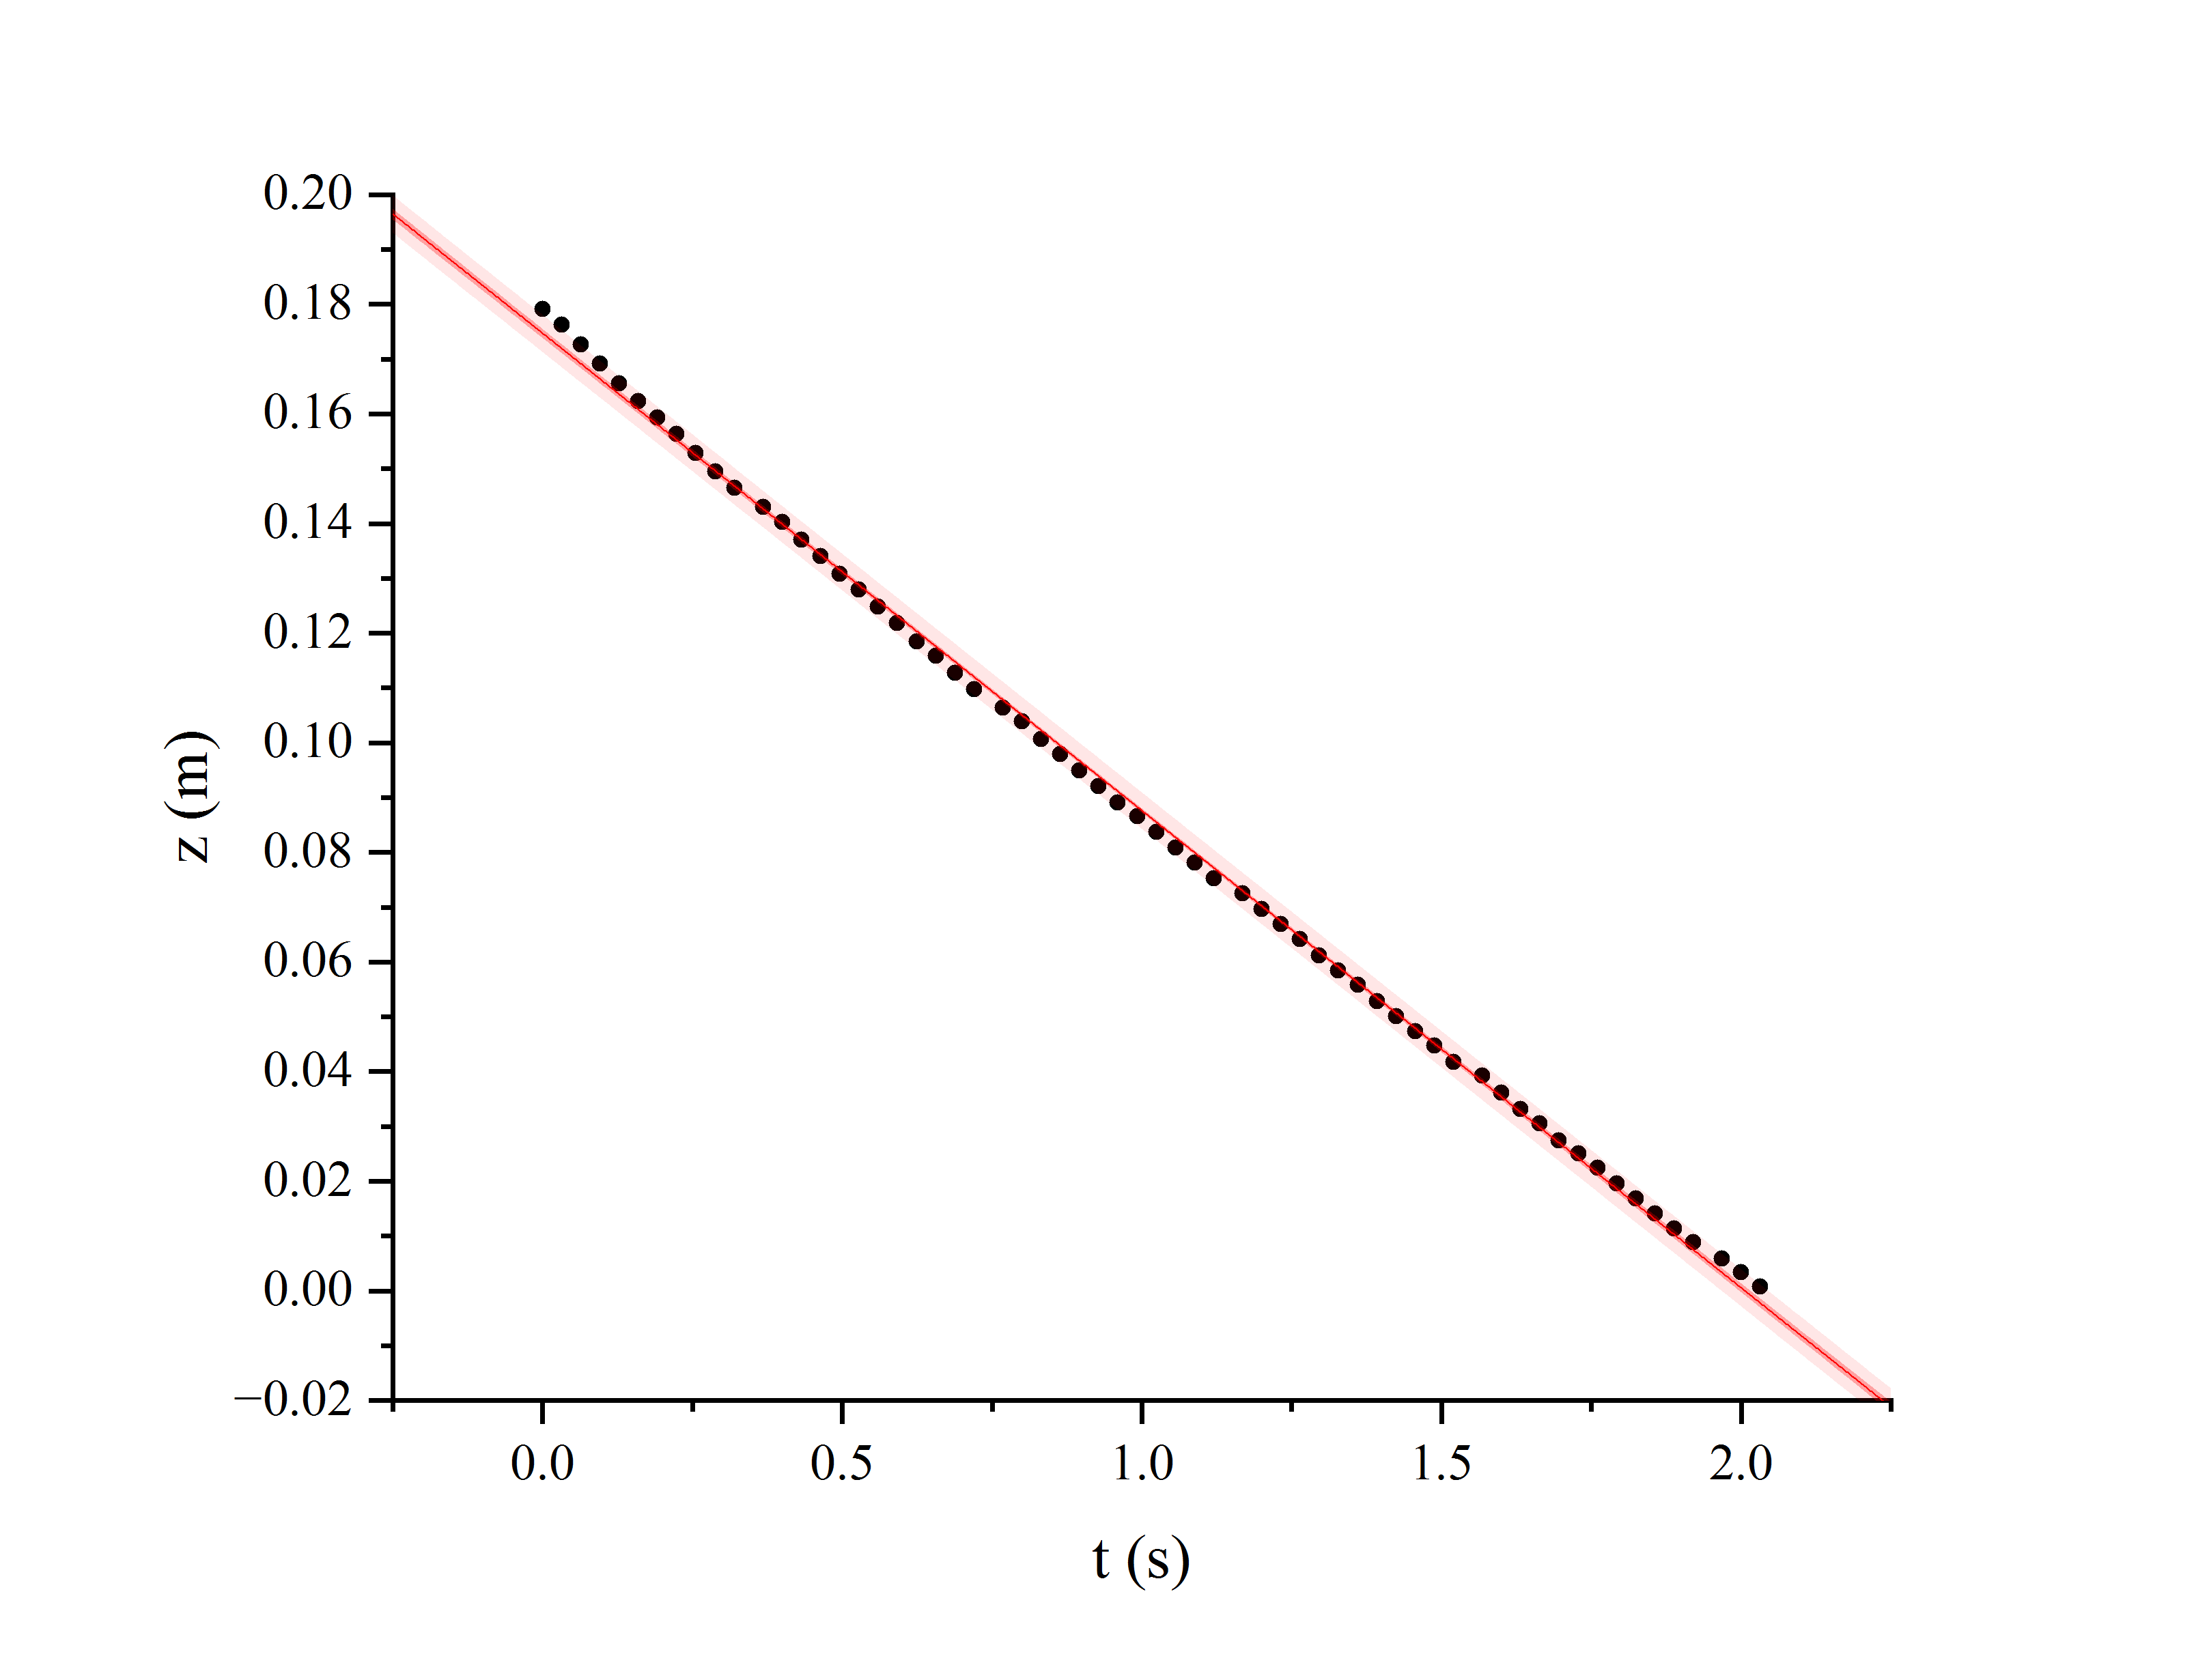
\includegraphics[trim={1.5cm 0.6cm 2cm 1cm},clip,width=\textwidth]{img/reg-p.png}
  \caption{\emph{
    In rosso la retta di regressione, in rosa la sua regione di incertezza.
  }}
\end{figure}

\emph{
  \textbf{Osservazione.} Come si può notare, l'andamento dei dati mostrati qui
  è ben descritto dalla retta: riteniamo che quindi, in questo caso, la sferetta
  abbia raggiunto la velocità limite prima di oltrepassare il primo traguardo.
}

\emph{
  Il gruppo di lavoro ha verificato in questo modo l'ipotesi (1.), osservando
  attentamente la distribuzione dei punti in ogni grafico: nessuno di questi
  ha mai mostrato una deviazione significativa dal modello lineare.
}

\pagebreak
Di seguito riportiamo le distribuzioni delle velocità per ogni classe
di sferette, di entrambi i giorni:
\vspace{-5mm}
\begin{center}
  \begin{figure}[H]
    % <v>^
    \centering
    \subfloat[][
      Primo giorno: piccole ($N=12$)

      $\overline{v}=(8.738\pm0.016)\cdot10^{-2}\,\unit{m\per s}$
    ]{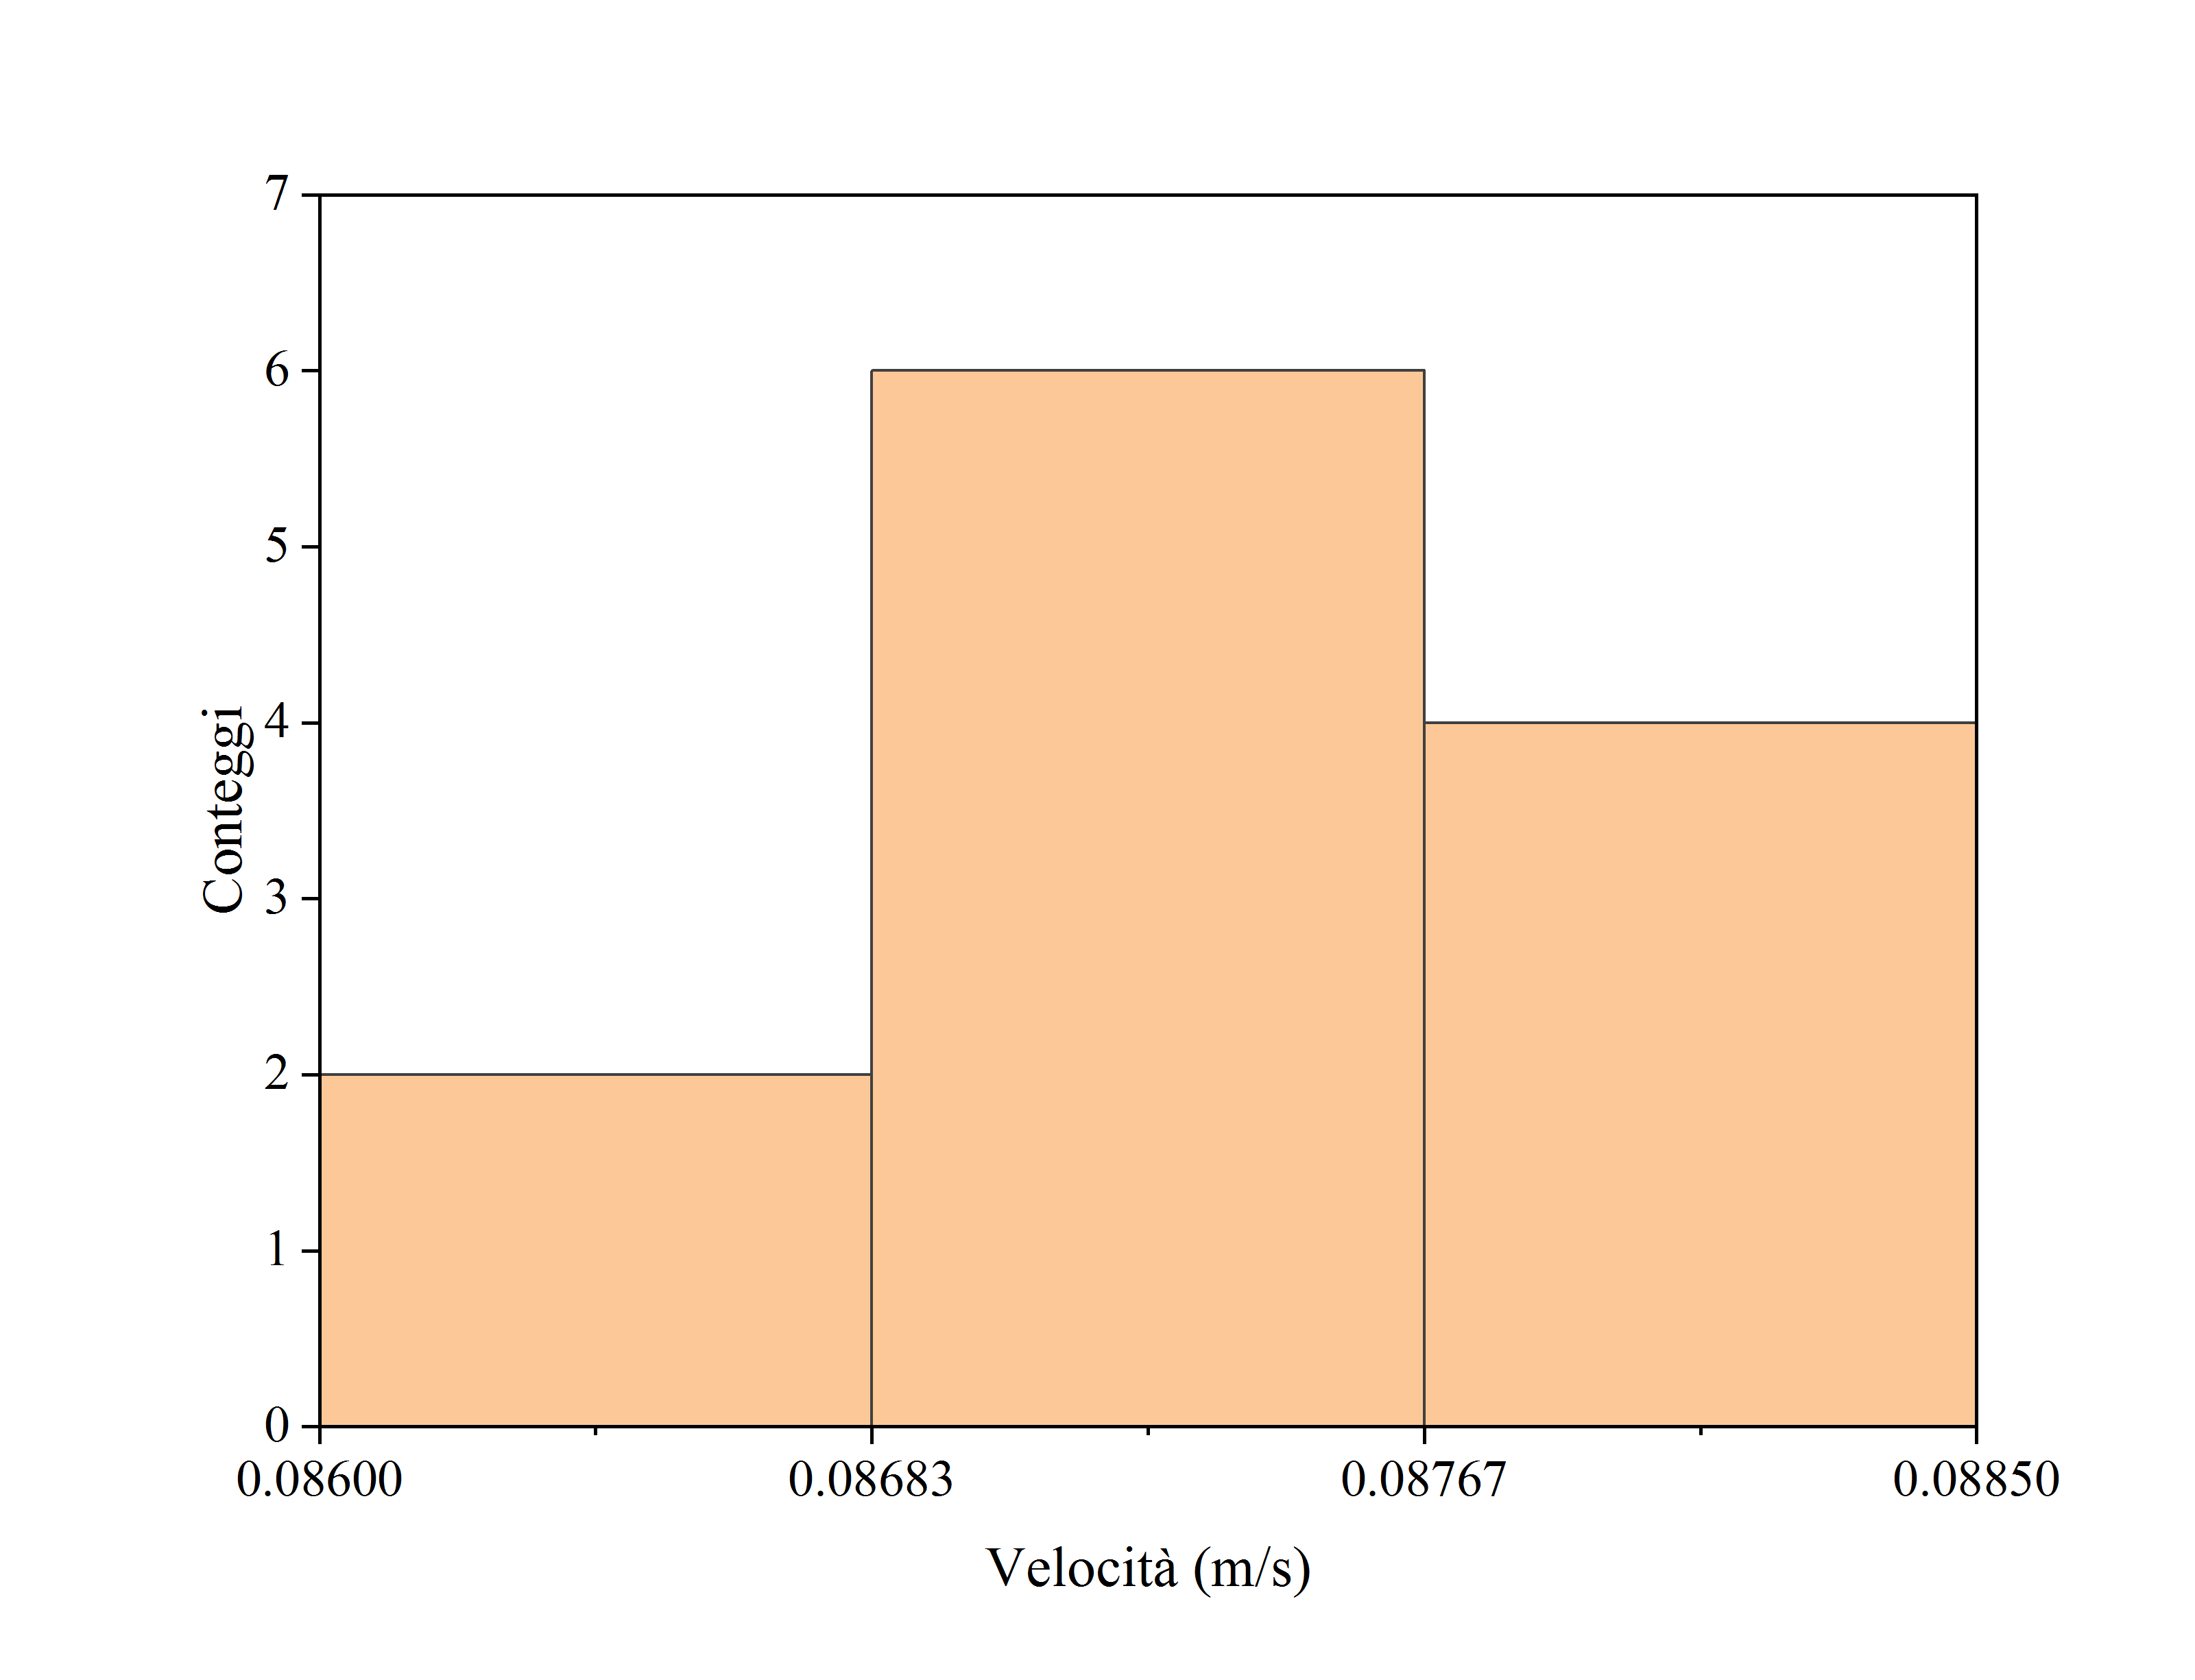
\includegraphics[trim={1cm 0.6cm 1cm 1cm},clip,width=.49\textwidth]{img/p1.png}}
    \hfil\subfloat[][
      Secondo giorno: piccole ($N=13$)

      $\overline{v}=(5.65\pm0.02)\cdot10^{-2}\,\unit{m\per s}$
    ]{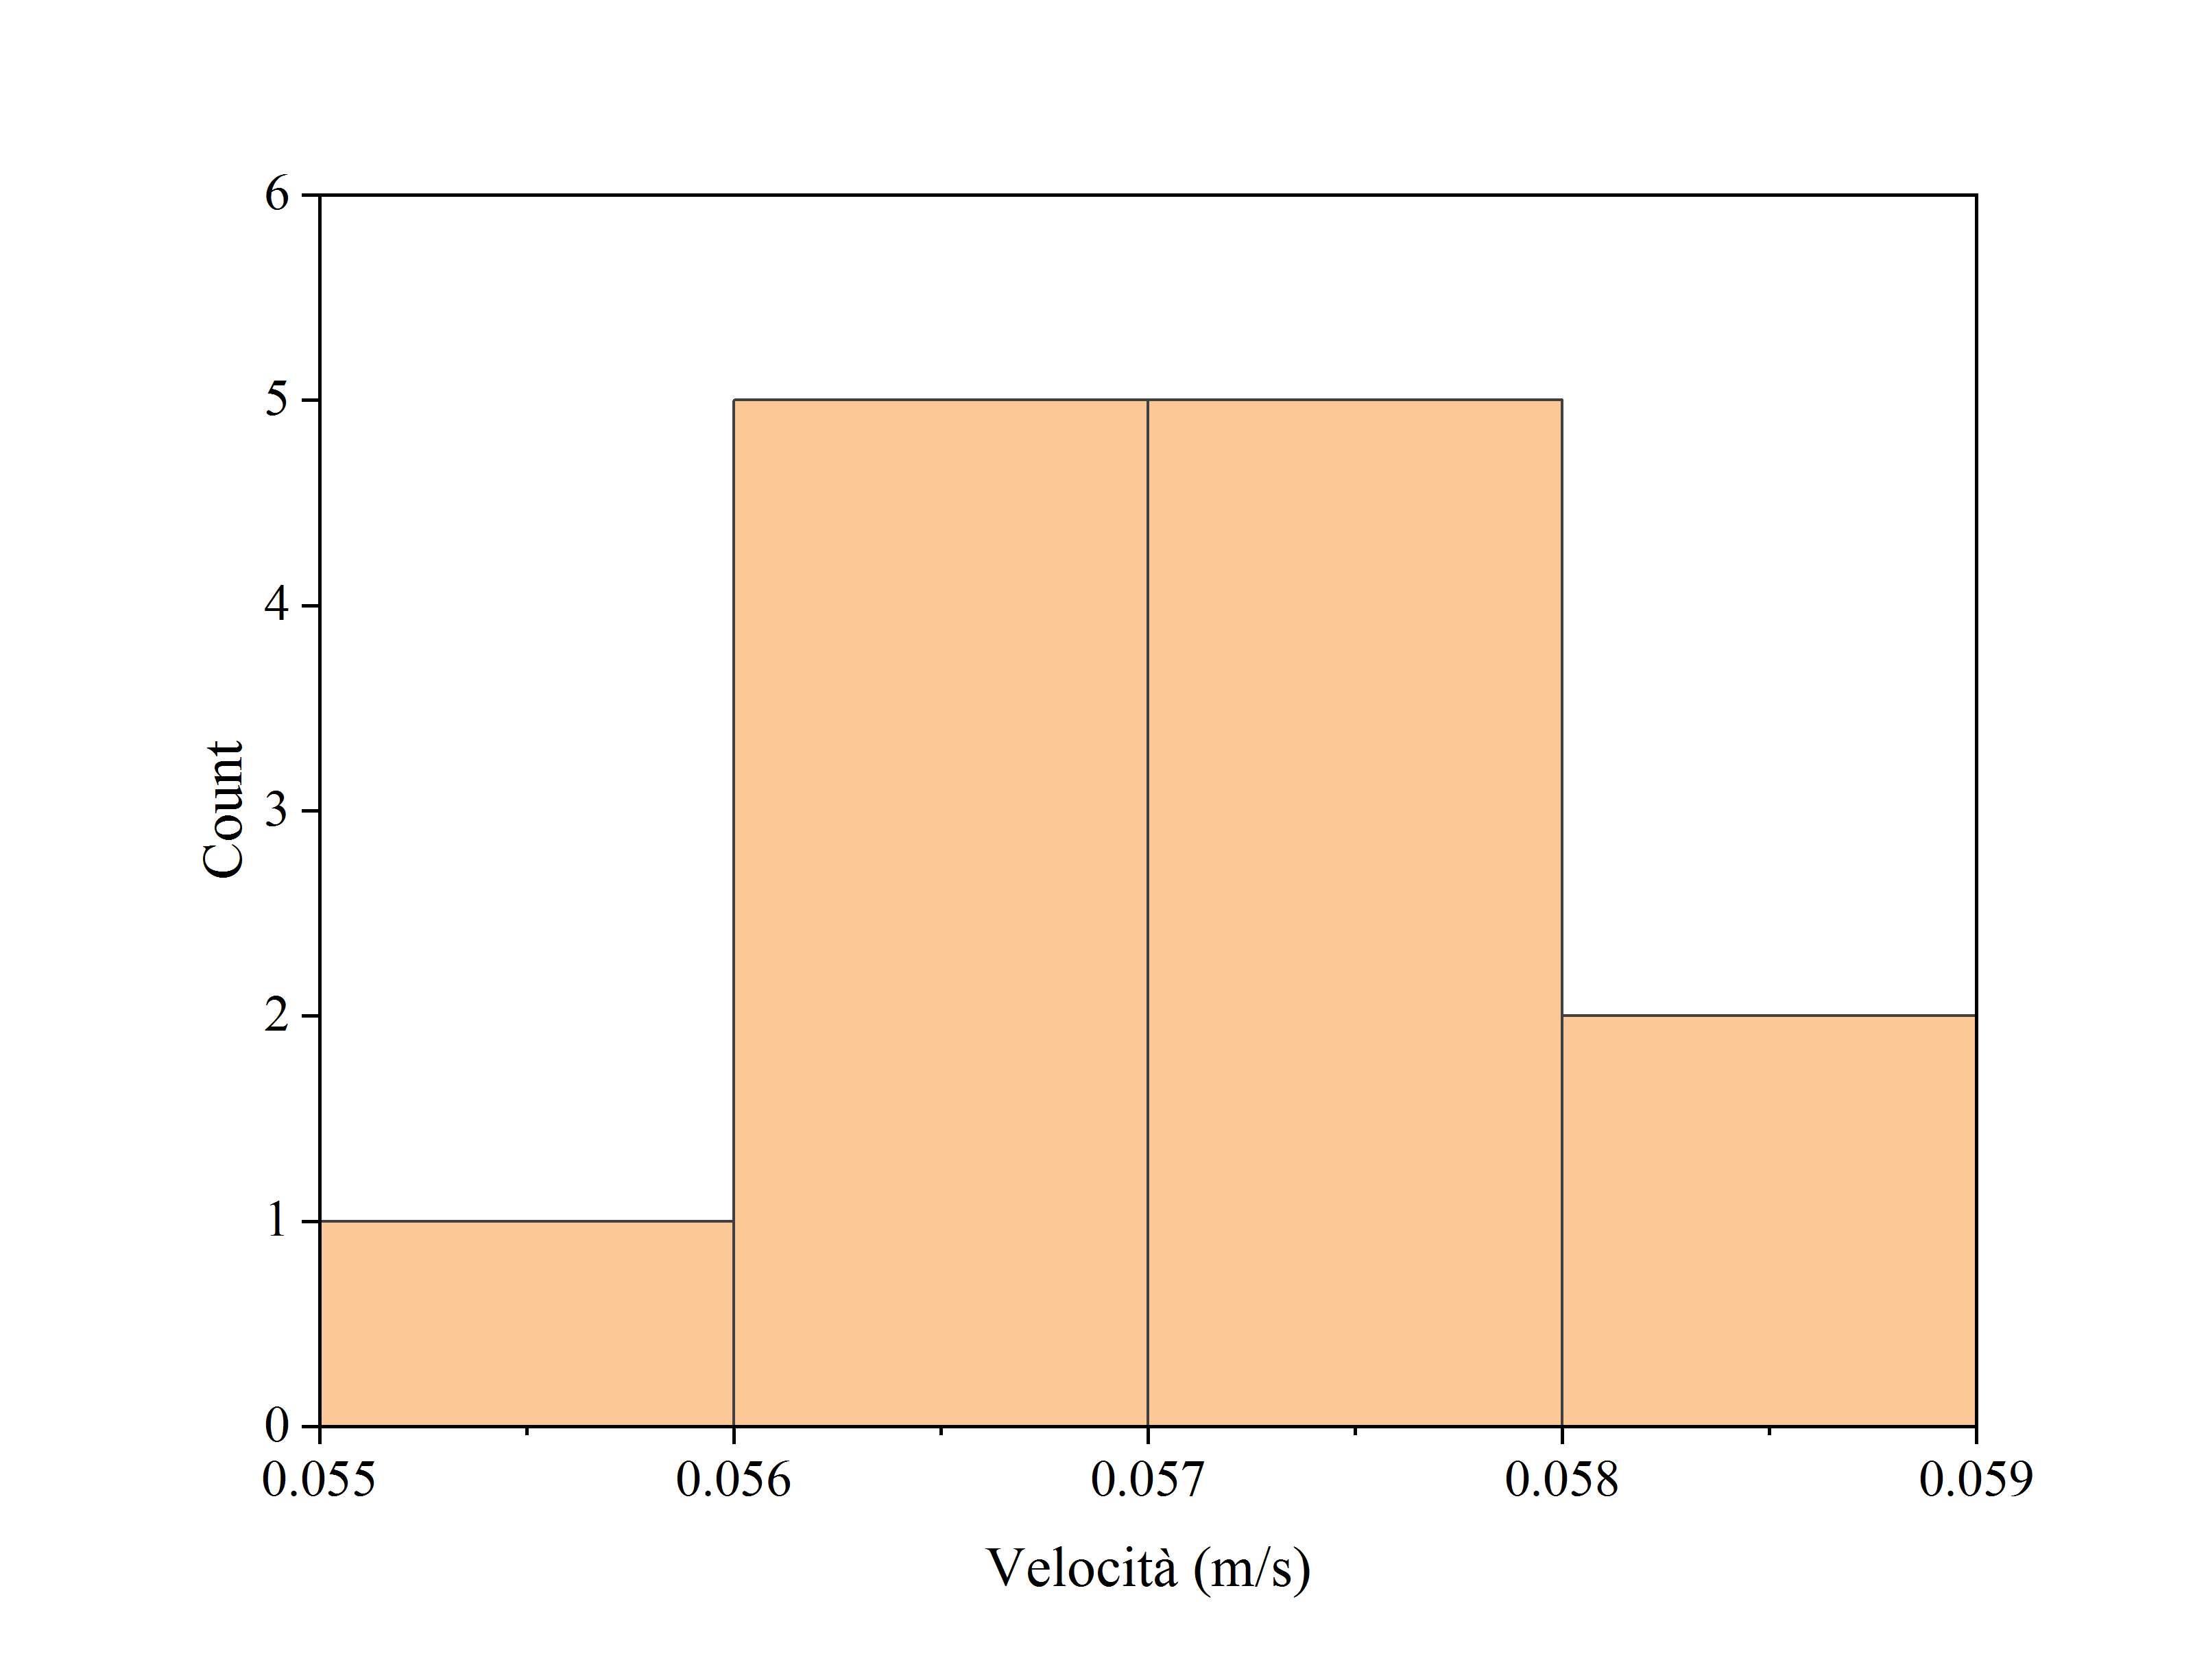
\includegraphics[trim={1cm 0.6cm 1cm 1cm},clip,width=.49\textwidth]{img/p2.png}}
    \hfil\subfloat[][
      Primo giorno: medie ($N=23$)

      $\overline{v}=(12.97\pm0.03)\cdot10^{-2}\,\unit{m\per s}$
    ]{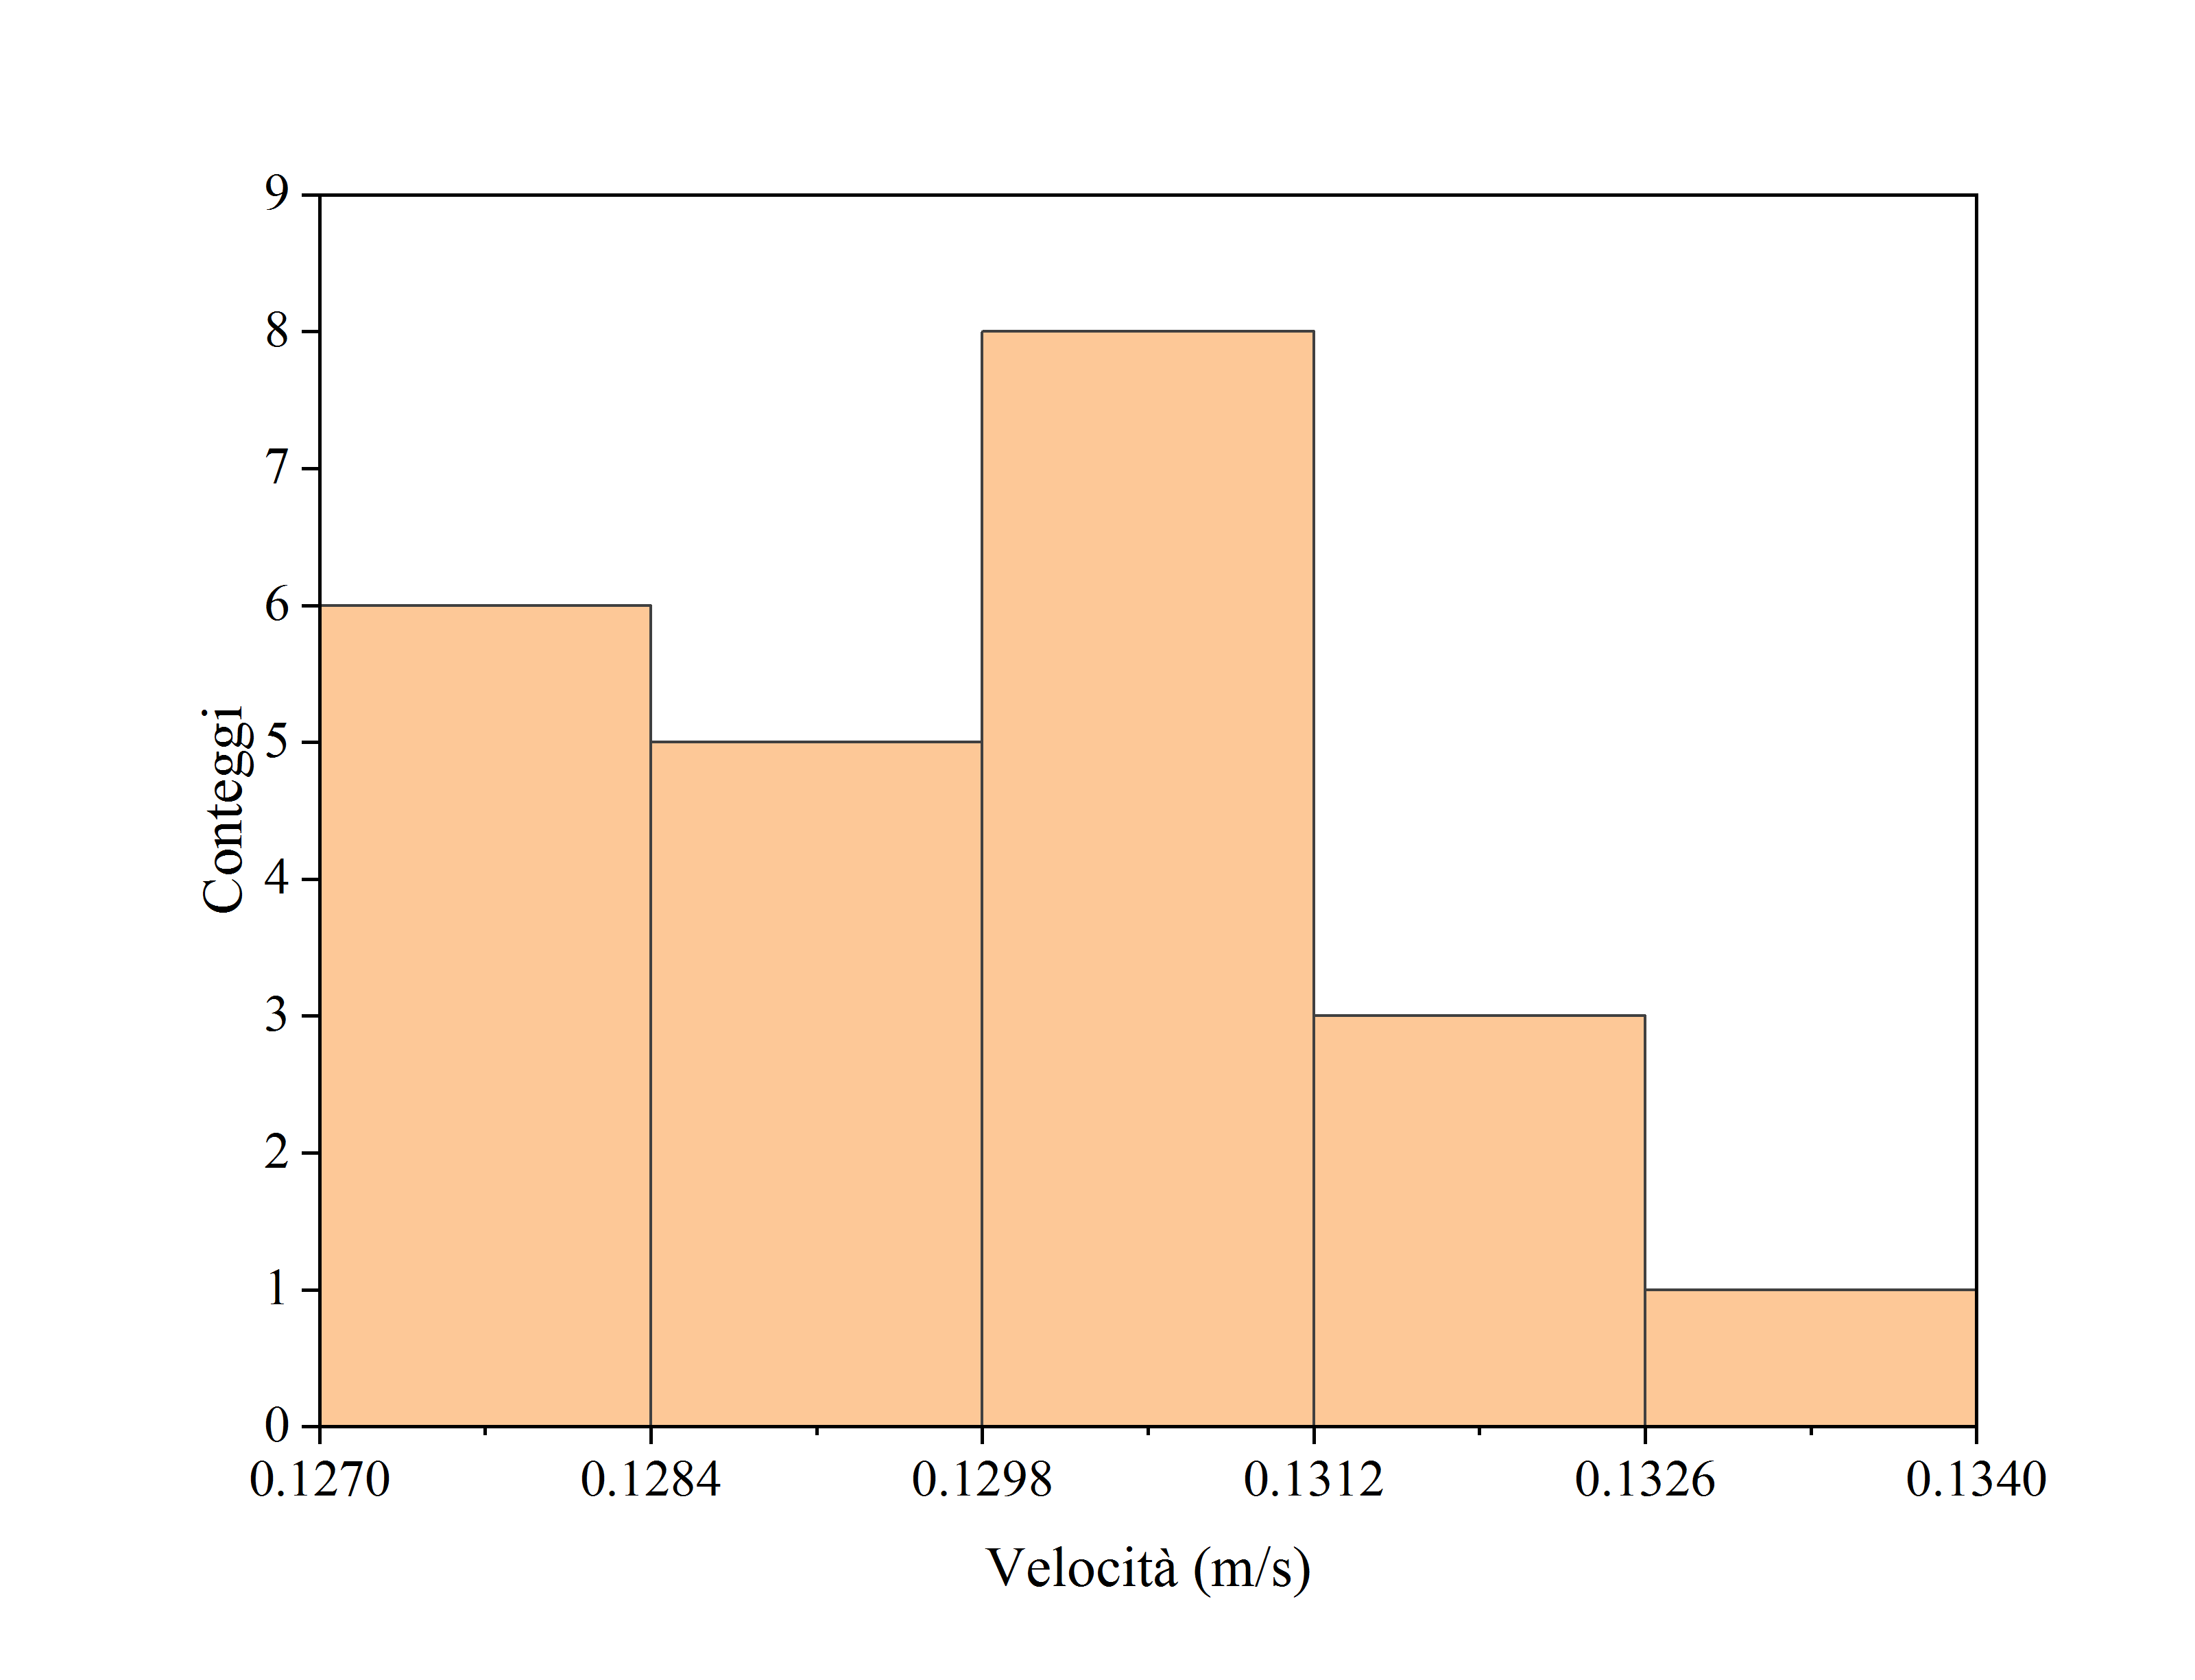
\includegraphics[trim={1cm 0.6cm 1cm 1cm},clip,width=.49\textwidth]{img/m1.png}}
    \hfil\subfloat[][
      Secondo giorno: medie ($N=23$)

      $\overline{v}=(8.61\pm0.04)\cdot10^{-2}\,\unit{m\per s}$
    ]{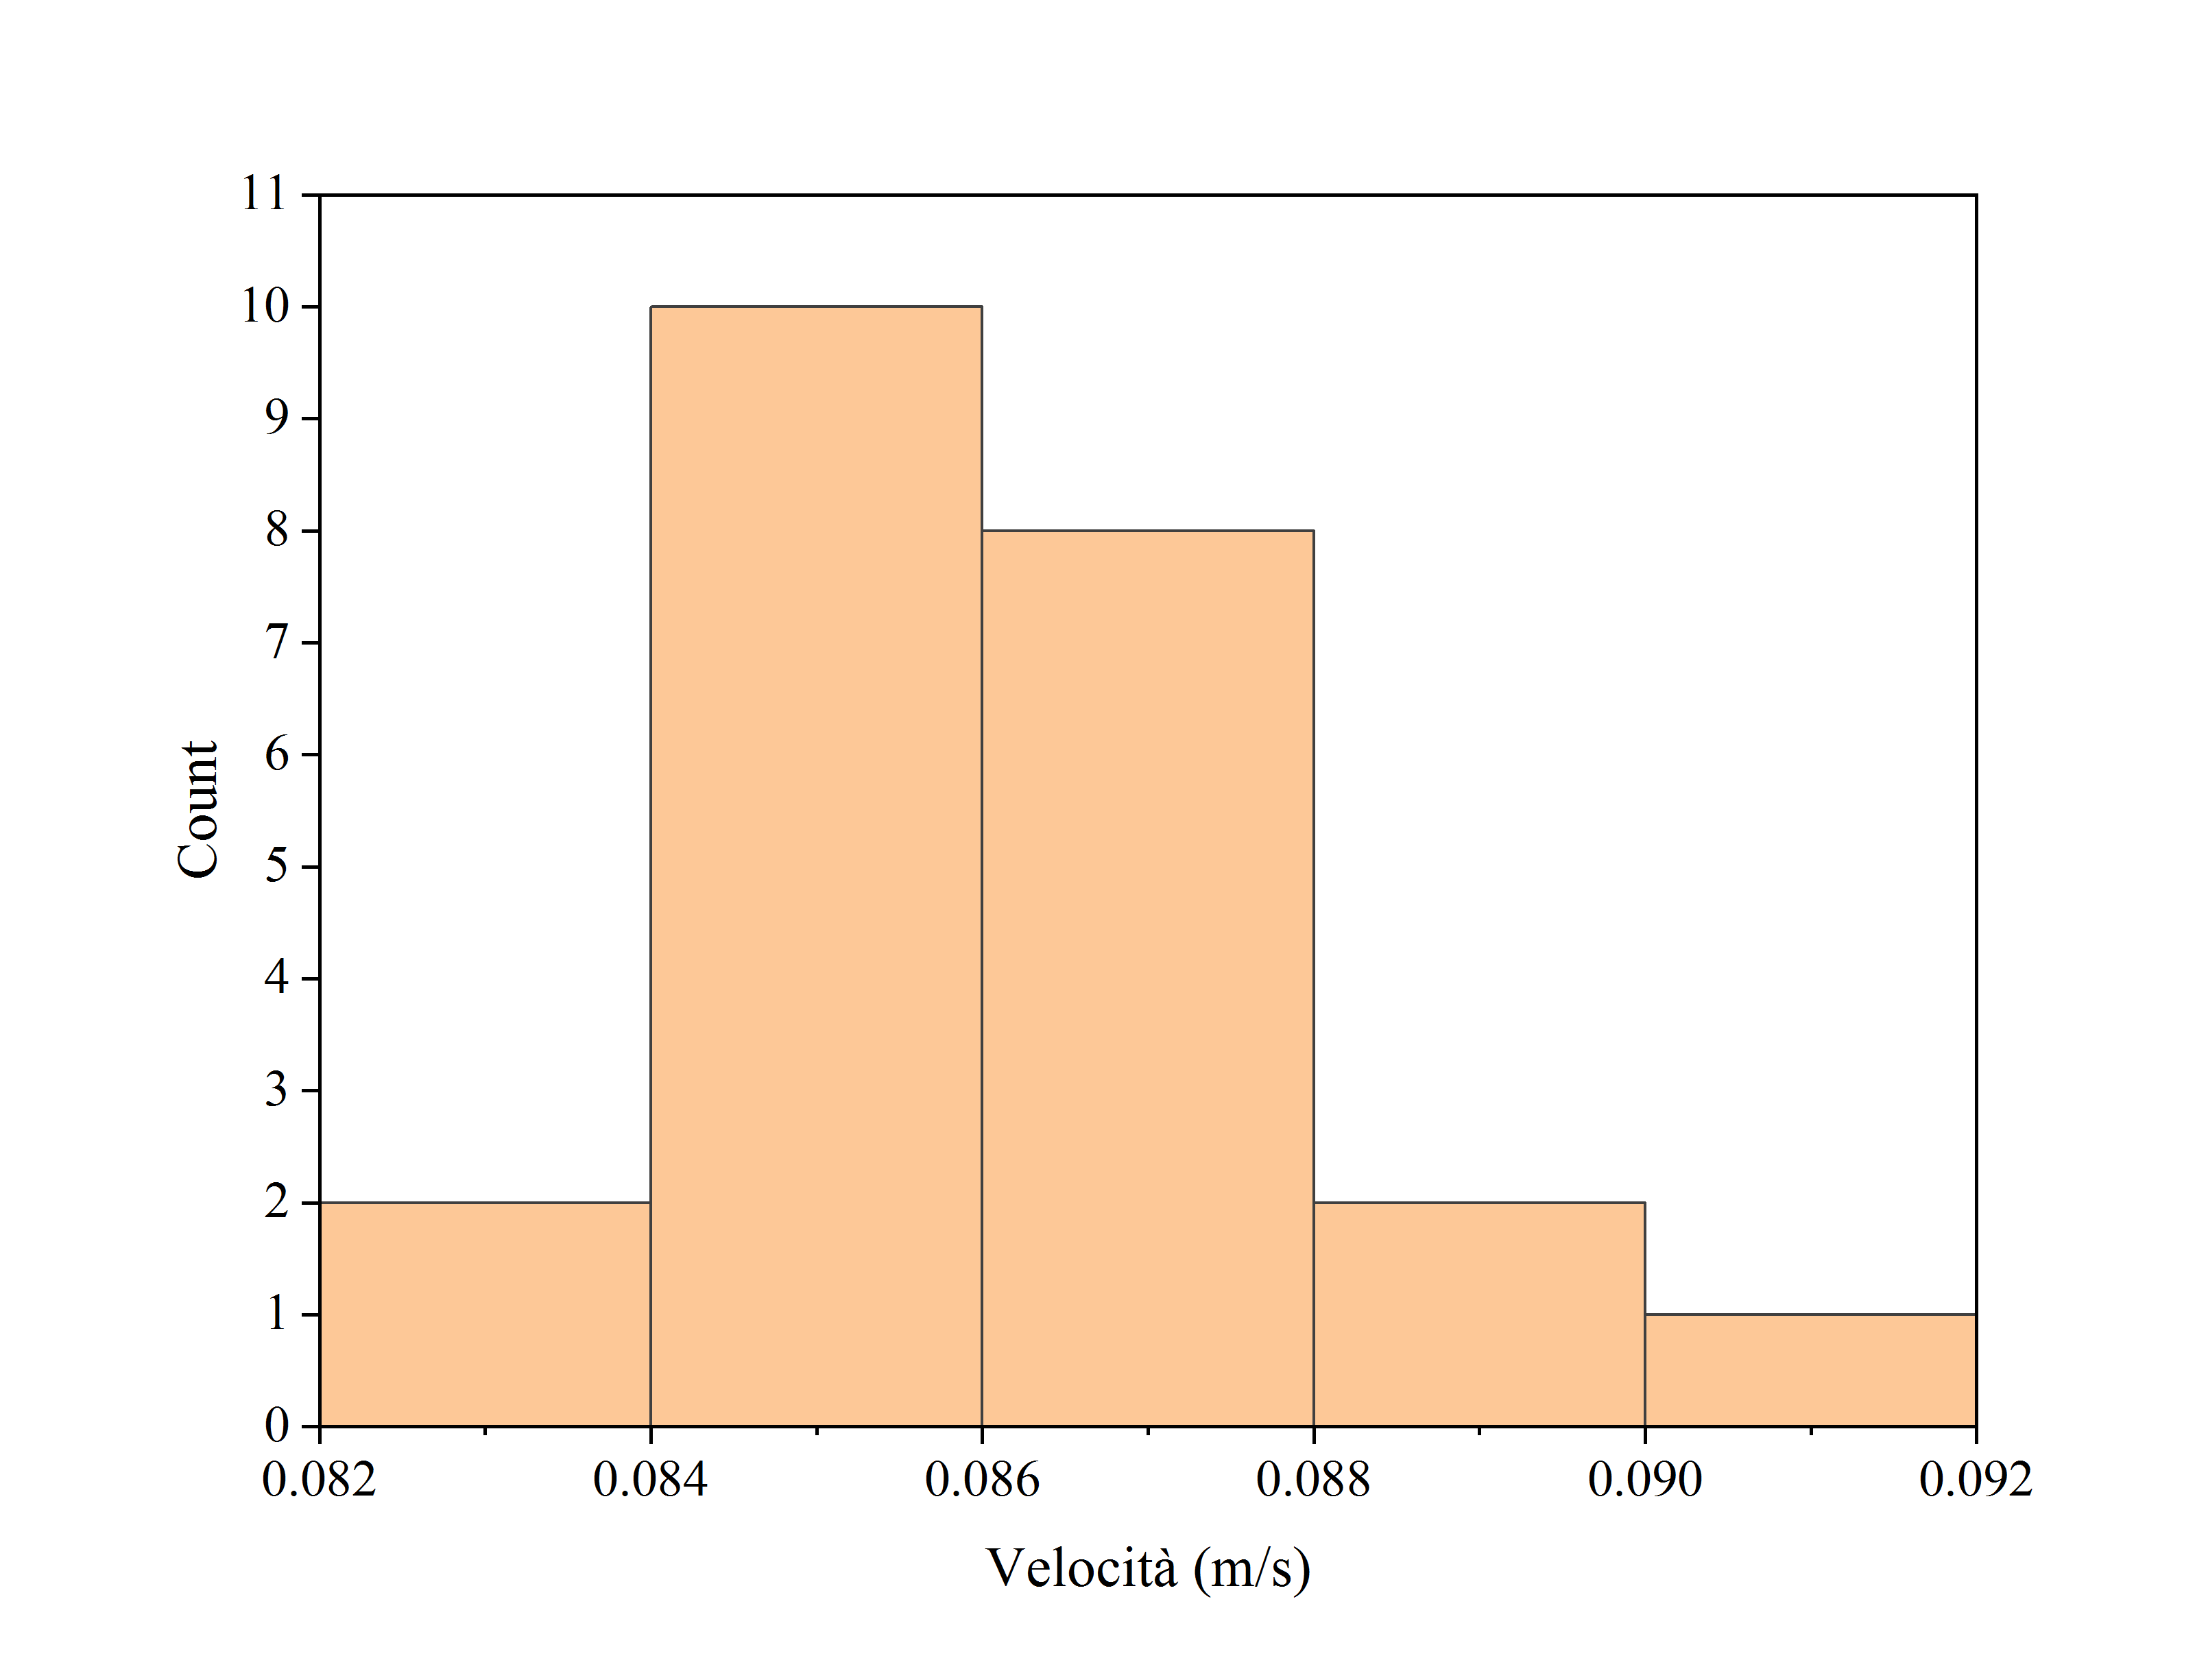
\includegraphics[trim={1cm 0.6cm 1cm 1cm},clip,width=.49\textwidth]{img/m2.png}}
    \hfil\subfloat[][
      Primo giorno: grandi ($N=32$)

      $\overline{v}=(19.58\pm0.05)\cdot10^{-2}\,\unit{m\per s}$
    ]{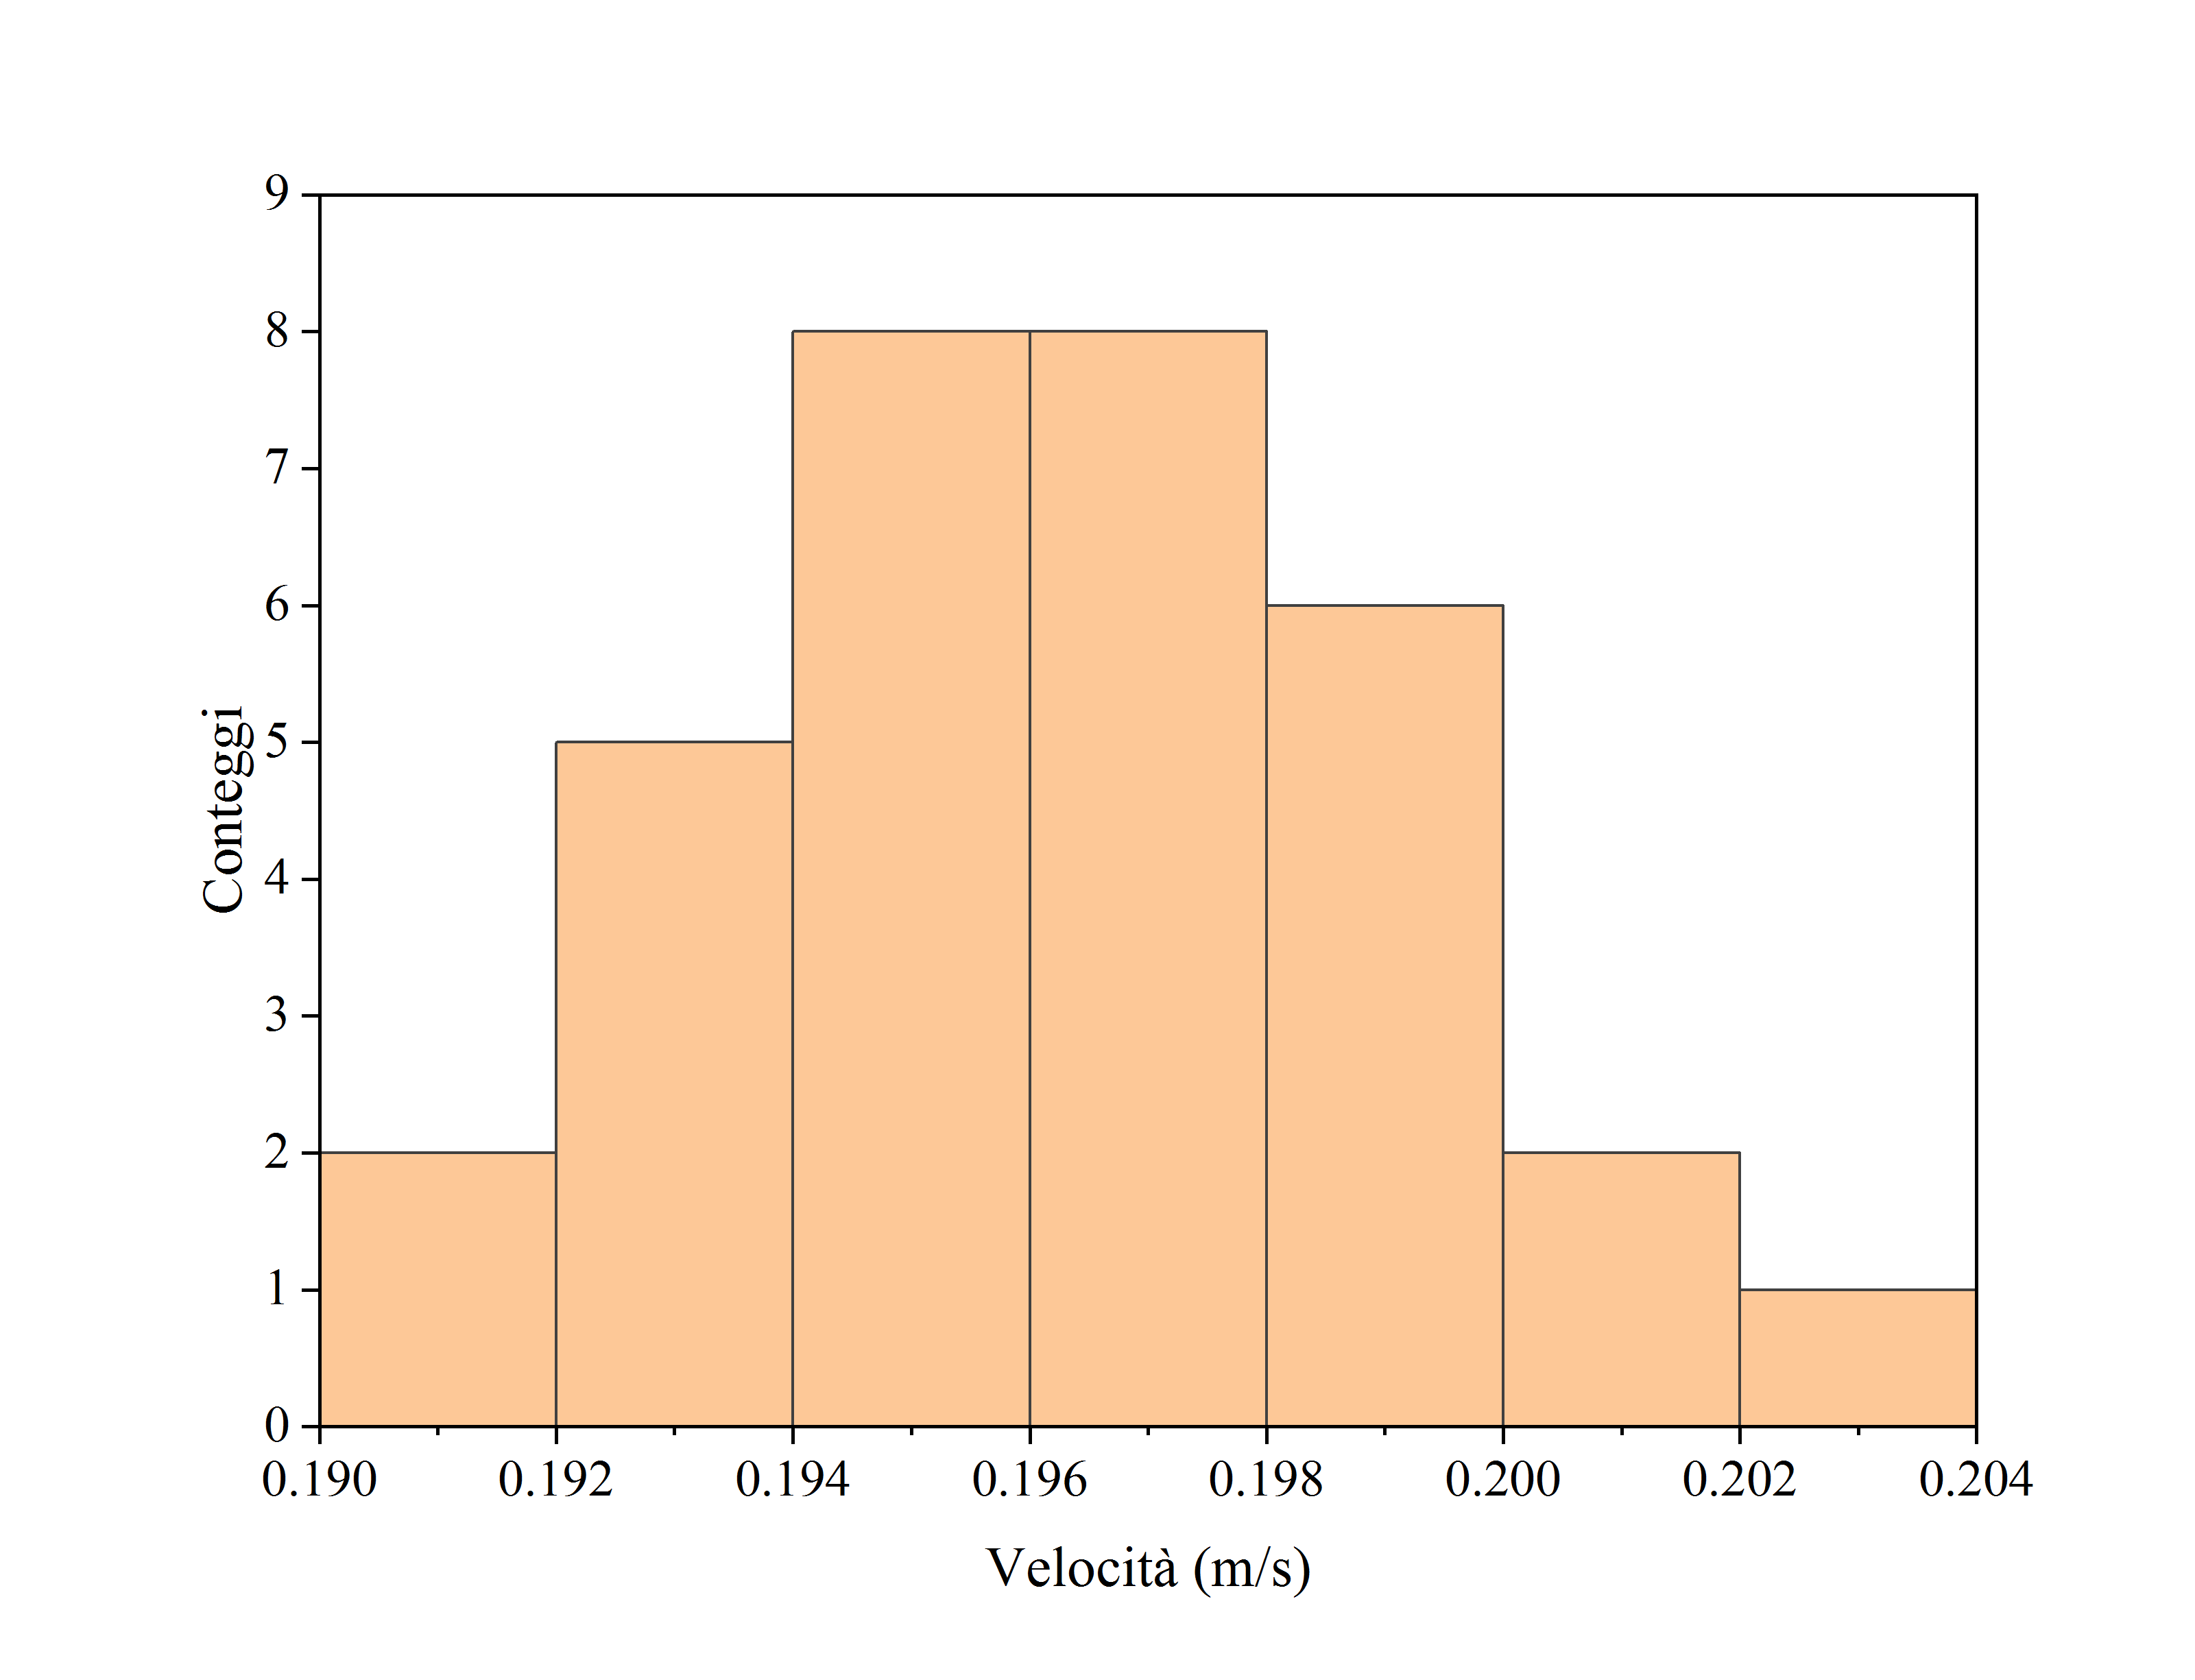
\includegraphics[trim={1cm 0.6cm 1cm 1cm},clip,width=.49\textwidth]{img/g1.png}}
    \hfil\subfloat[][
      Secondo giorno: grandi ($N=28$)

      $\overline{v}=(14.48\pm0.06)\cdot10^{-2}\,\unit{m\per s}$
    ]{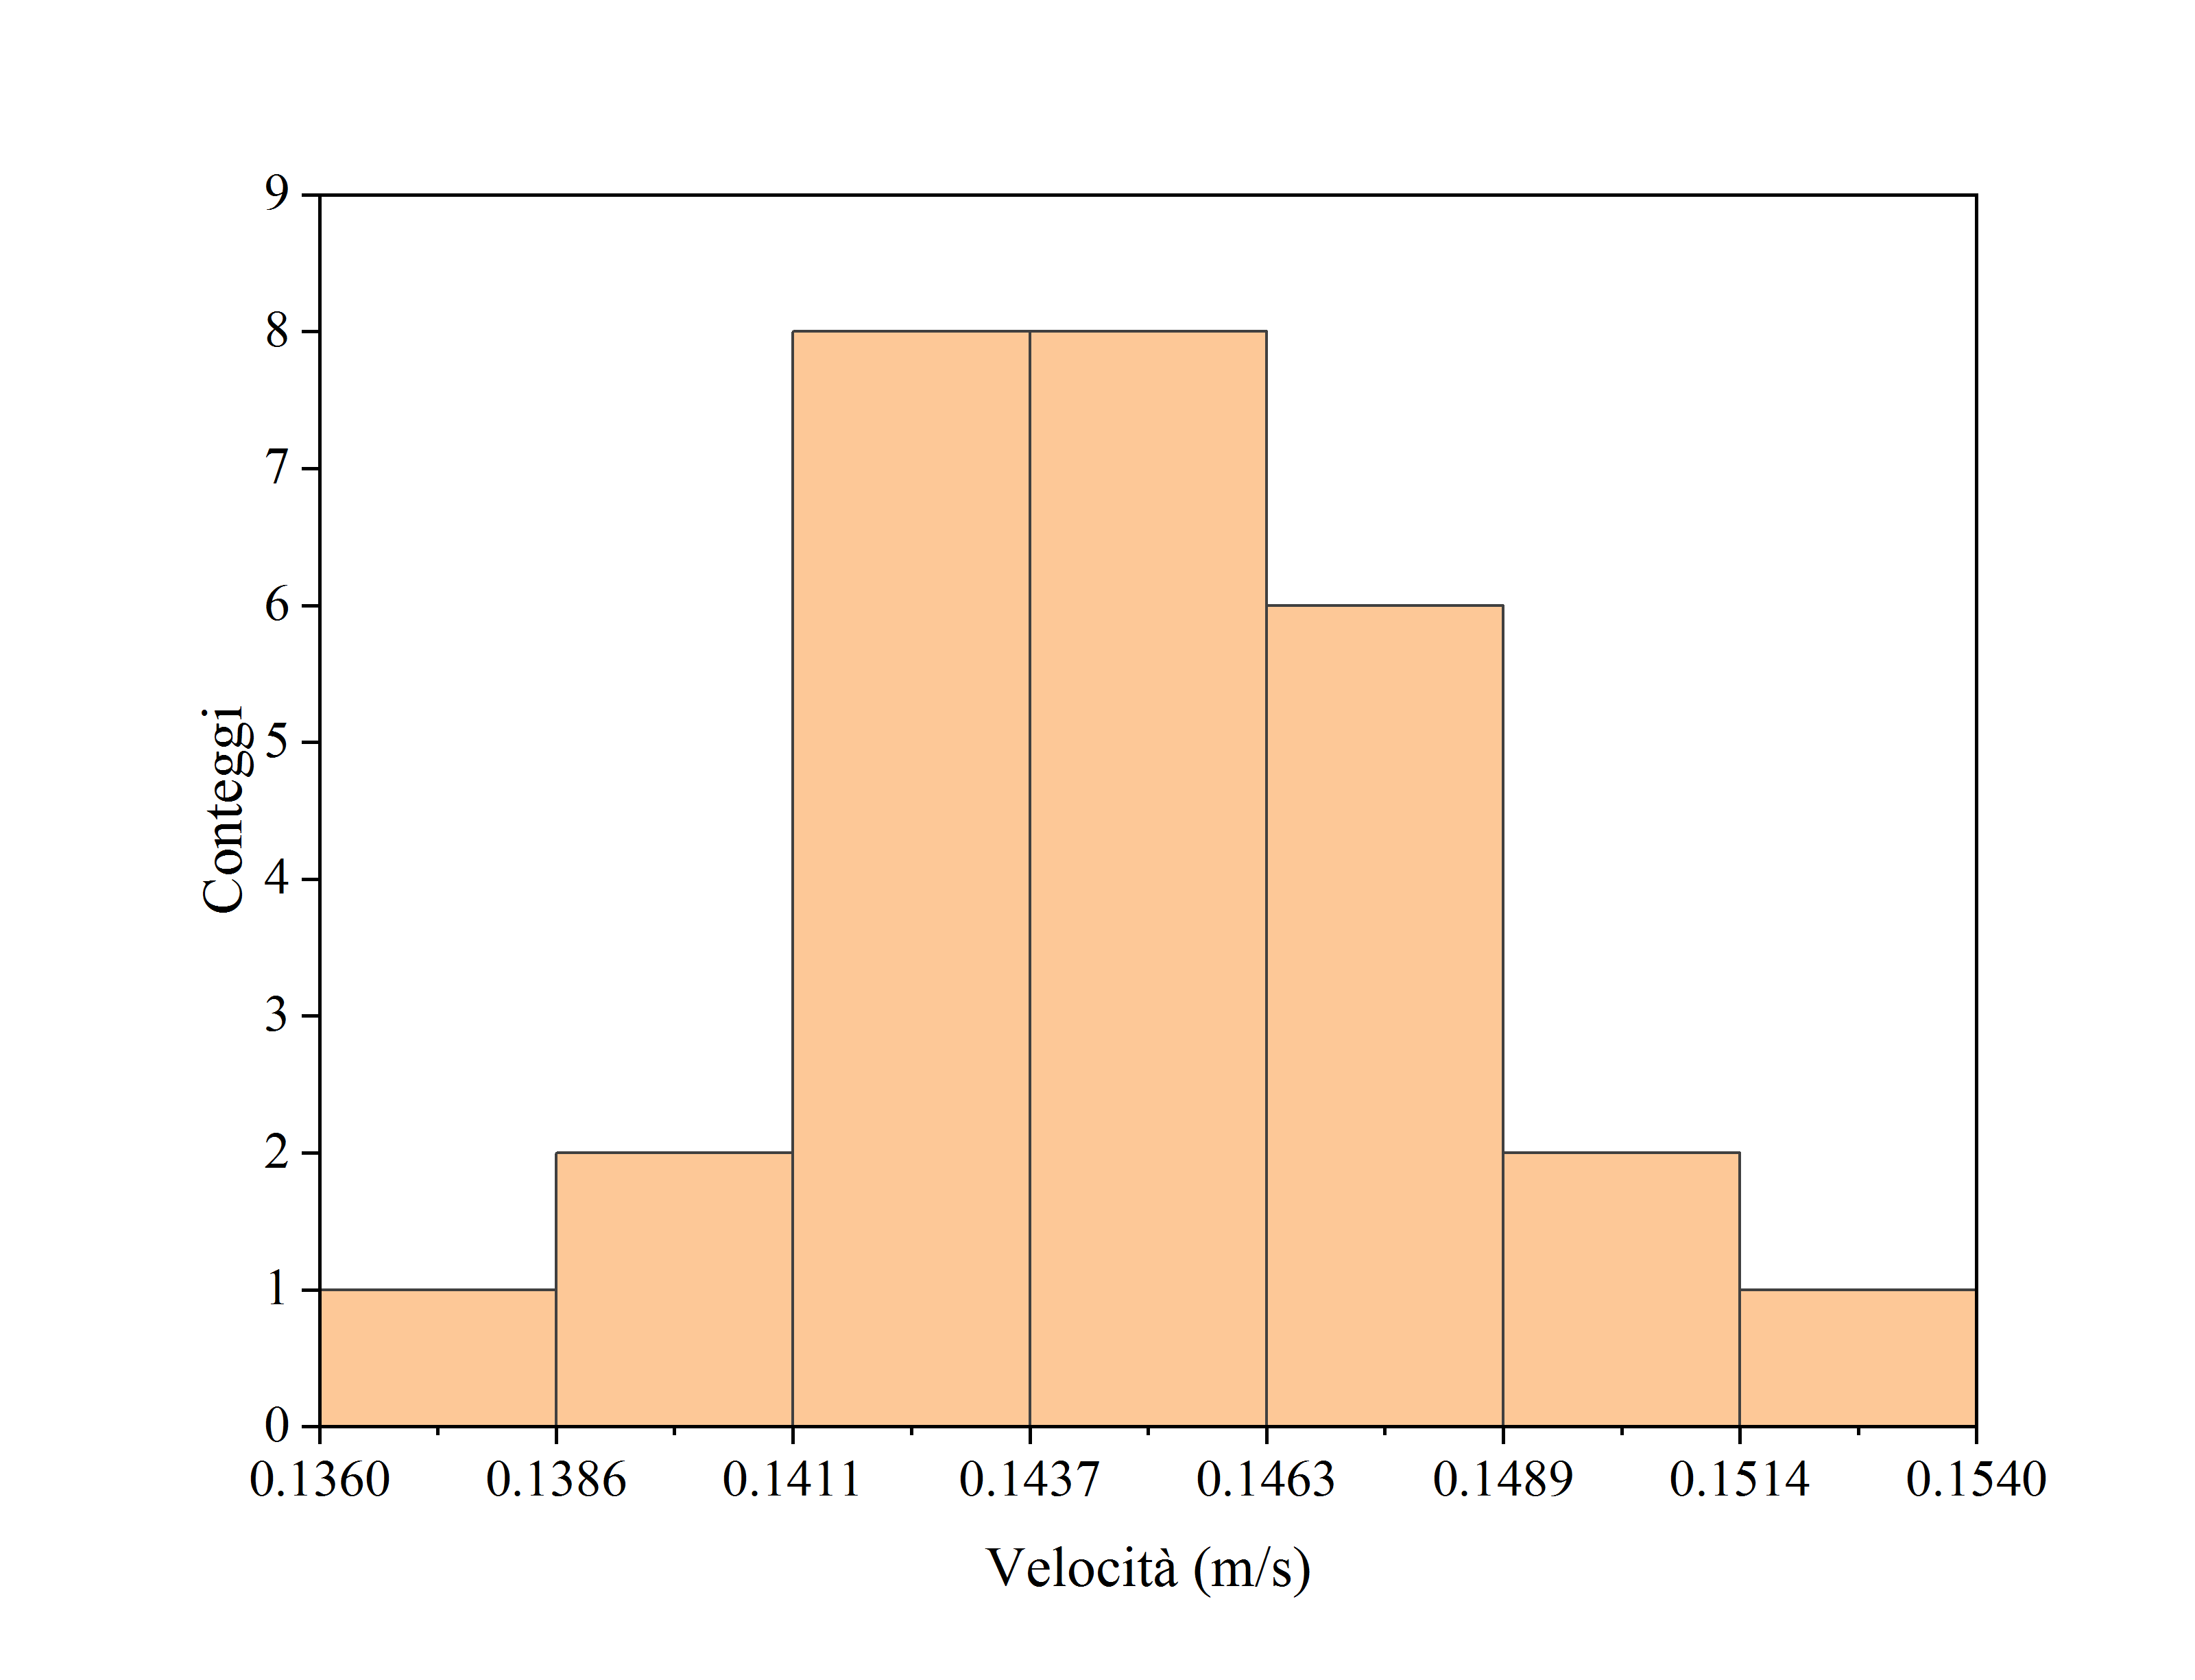
\includegraphics[trim={1cm 0.6cm 1cm 1cm},clip,width=.49\textwidth]{img/g2.png}}
  \end{figure}
\end{center}

\pagebreak
\subsection{Modello di $\rho(T)$ ed $\eta(T)$ per i liquidi puri}
Poiché la densità e la viscosità di un fluido reale dipendono
dalla temperatura, il gruppo di lavoro ha ottenuto opportuno
applicare un modello empirico.
% TODO: Citare le fonti
% TODO: Citare i limiti del modello
\[\begin{aligned}
  \eta_\text{acqua}(T\,\,\unit{\degree C}) &= 1.79\cdot\exp{\!\left(
    \frac{-(1230 + T)\cdot T}{36100 + 360\,T}
  \right)}\,\unit{mPa\,s} \\
  \eta_\text{glicerina}(T\,\,\unit{\degree C}) &= 12100\cdot\exp{\!\left(
    \frac{-(1233 + T)\cdot T}{9900 + 70\,T}\right)}\,\unit{mPa\,s} \\
  \rho_\text{acqua}(T\,\,\unit{\degree C}) &= 1000 \left(
    1 - \left|\frac{T - 3.98}{615}\right|^{1.71} \right)\,\unit{kg \per m^3} \\
  \rho_\text{glicerina}(T\,\,\unit{\degree C}) &= \left(
    1273 - 0.612\,T \right)\,\unit{kg \per m^3}
\end{aligned}\]

Di seguito riportiamo i valori di queste grandezze, calcolati alle
due temperature $T_{\text{amb},1}$ e $T_{\text{amb},2}$:
\begin{center}
\begin{tblr}{
  colspec={ |cc|c|c| },
}
  % TODO: Ricalcolare gli errori con la formula giusta
  \hline
  $T_{\text{amb}}$ & $(\unit{\degree C})$
    & $24.6\pm0.2$ & $19.4\pm0.2$ \\
  \hline
  $\eta_\text{acqua}$ & $(\unit{mPa\,s})$
    & $0.901\pm0.006$ & $1.020\pm0.007$ \\
  \hline[dashed]
  $\eta_\text{glicerina}$ & $(\unit{mPa\,s})$
    & $845\pm21$ & $1398\pm35$ \\
  \hline[dashed]
  $\rho_\text{acqua}$ & $(\unit{kg \per m^3})$
    & $996.99\pm0.05$ & $998.17\pm0.04$ \\
  \hline[dashed]
  $\rho_\text{glicerina}$ & $(\unit{kg \per m^3})$
    & $1257.94\pm0.12$ & $1261.13\pm0.12$ \\
  \hline
\end{tblr}
\end{center}

\subsection{Misura di $\eta$}
Ricordiamo la relazione tra $\overline{v}_k$ e $\overline{r}_k^2$:
\[
  \overline{v}_k = \xi\cdot\overline{r}_k^2
  \qquad\qquad\text{avendo posto}\qquad
  \xi = \frac{2g(\rho_\text{sf} - \rho_\text{sol})}{9\eta}
\]
Trattandosi di una relazione lineare, è possibile determinare una
retta di regressione, nella quale, poiché il modello lo richiedeva,
abbiamo fissato l'intercetta a 0.
Chiaramente, i dati dei due giorni devono essere trattati separatamente,
poiché $\rho_\text{sol}$ ed $\eta$ dipendono dalla temperatura ambiente.

Di seguito riportiamo i due grafici così ottenuti:

\vspace{-2mm}
\begin{figure}[H]
  \centering
  \subfloat[][
    Primo giorno

    $\xi=(8.738\pm0.016)\cdot10^{-2}\,\unit{m\cdot s}$
  ]{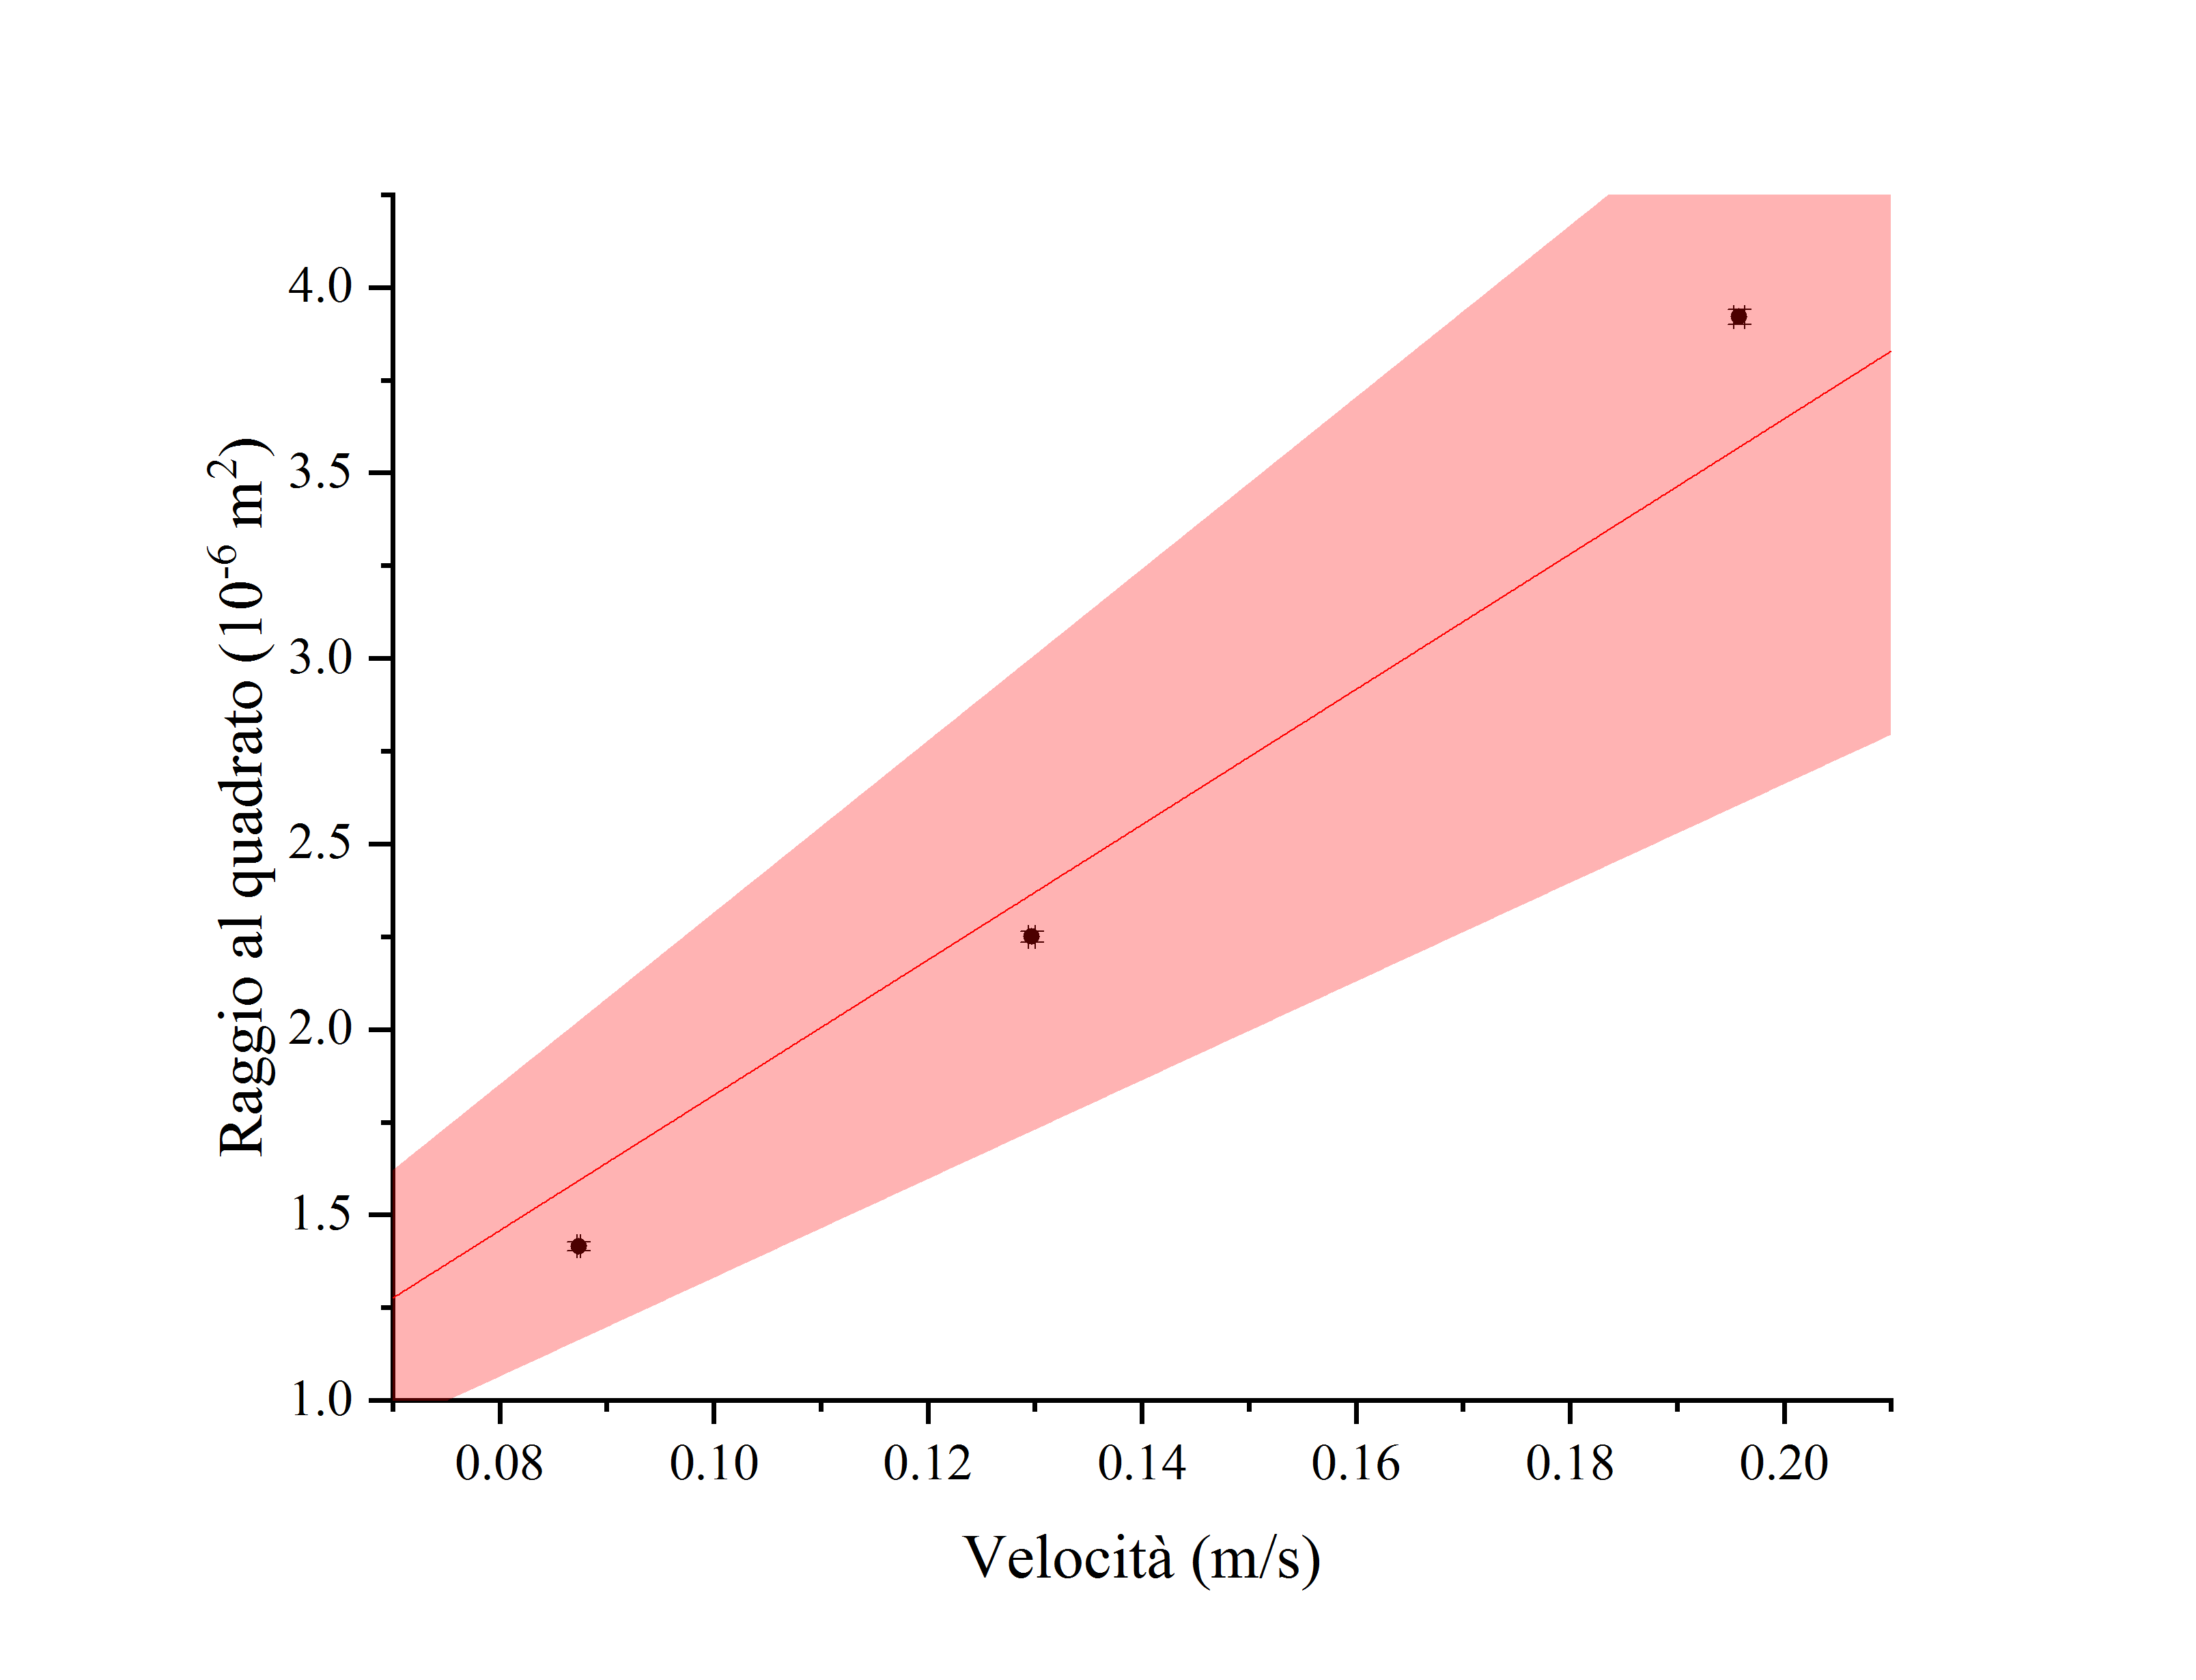
\includegraphics[trim={2.5cm 0.6cm 2.5cm 2.5cm},clip,width=.49\textwidth]{img/reg1.png}}
  \hfil\subfloat[][
    Secondo giorno

    $\xi=(5.65\pm0.02)\cdot10^{-2}\,\unit{m\cdot s}$
  ]{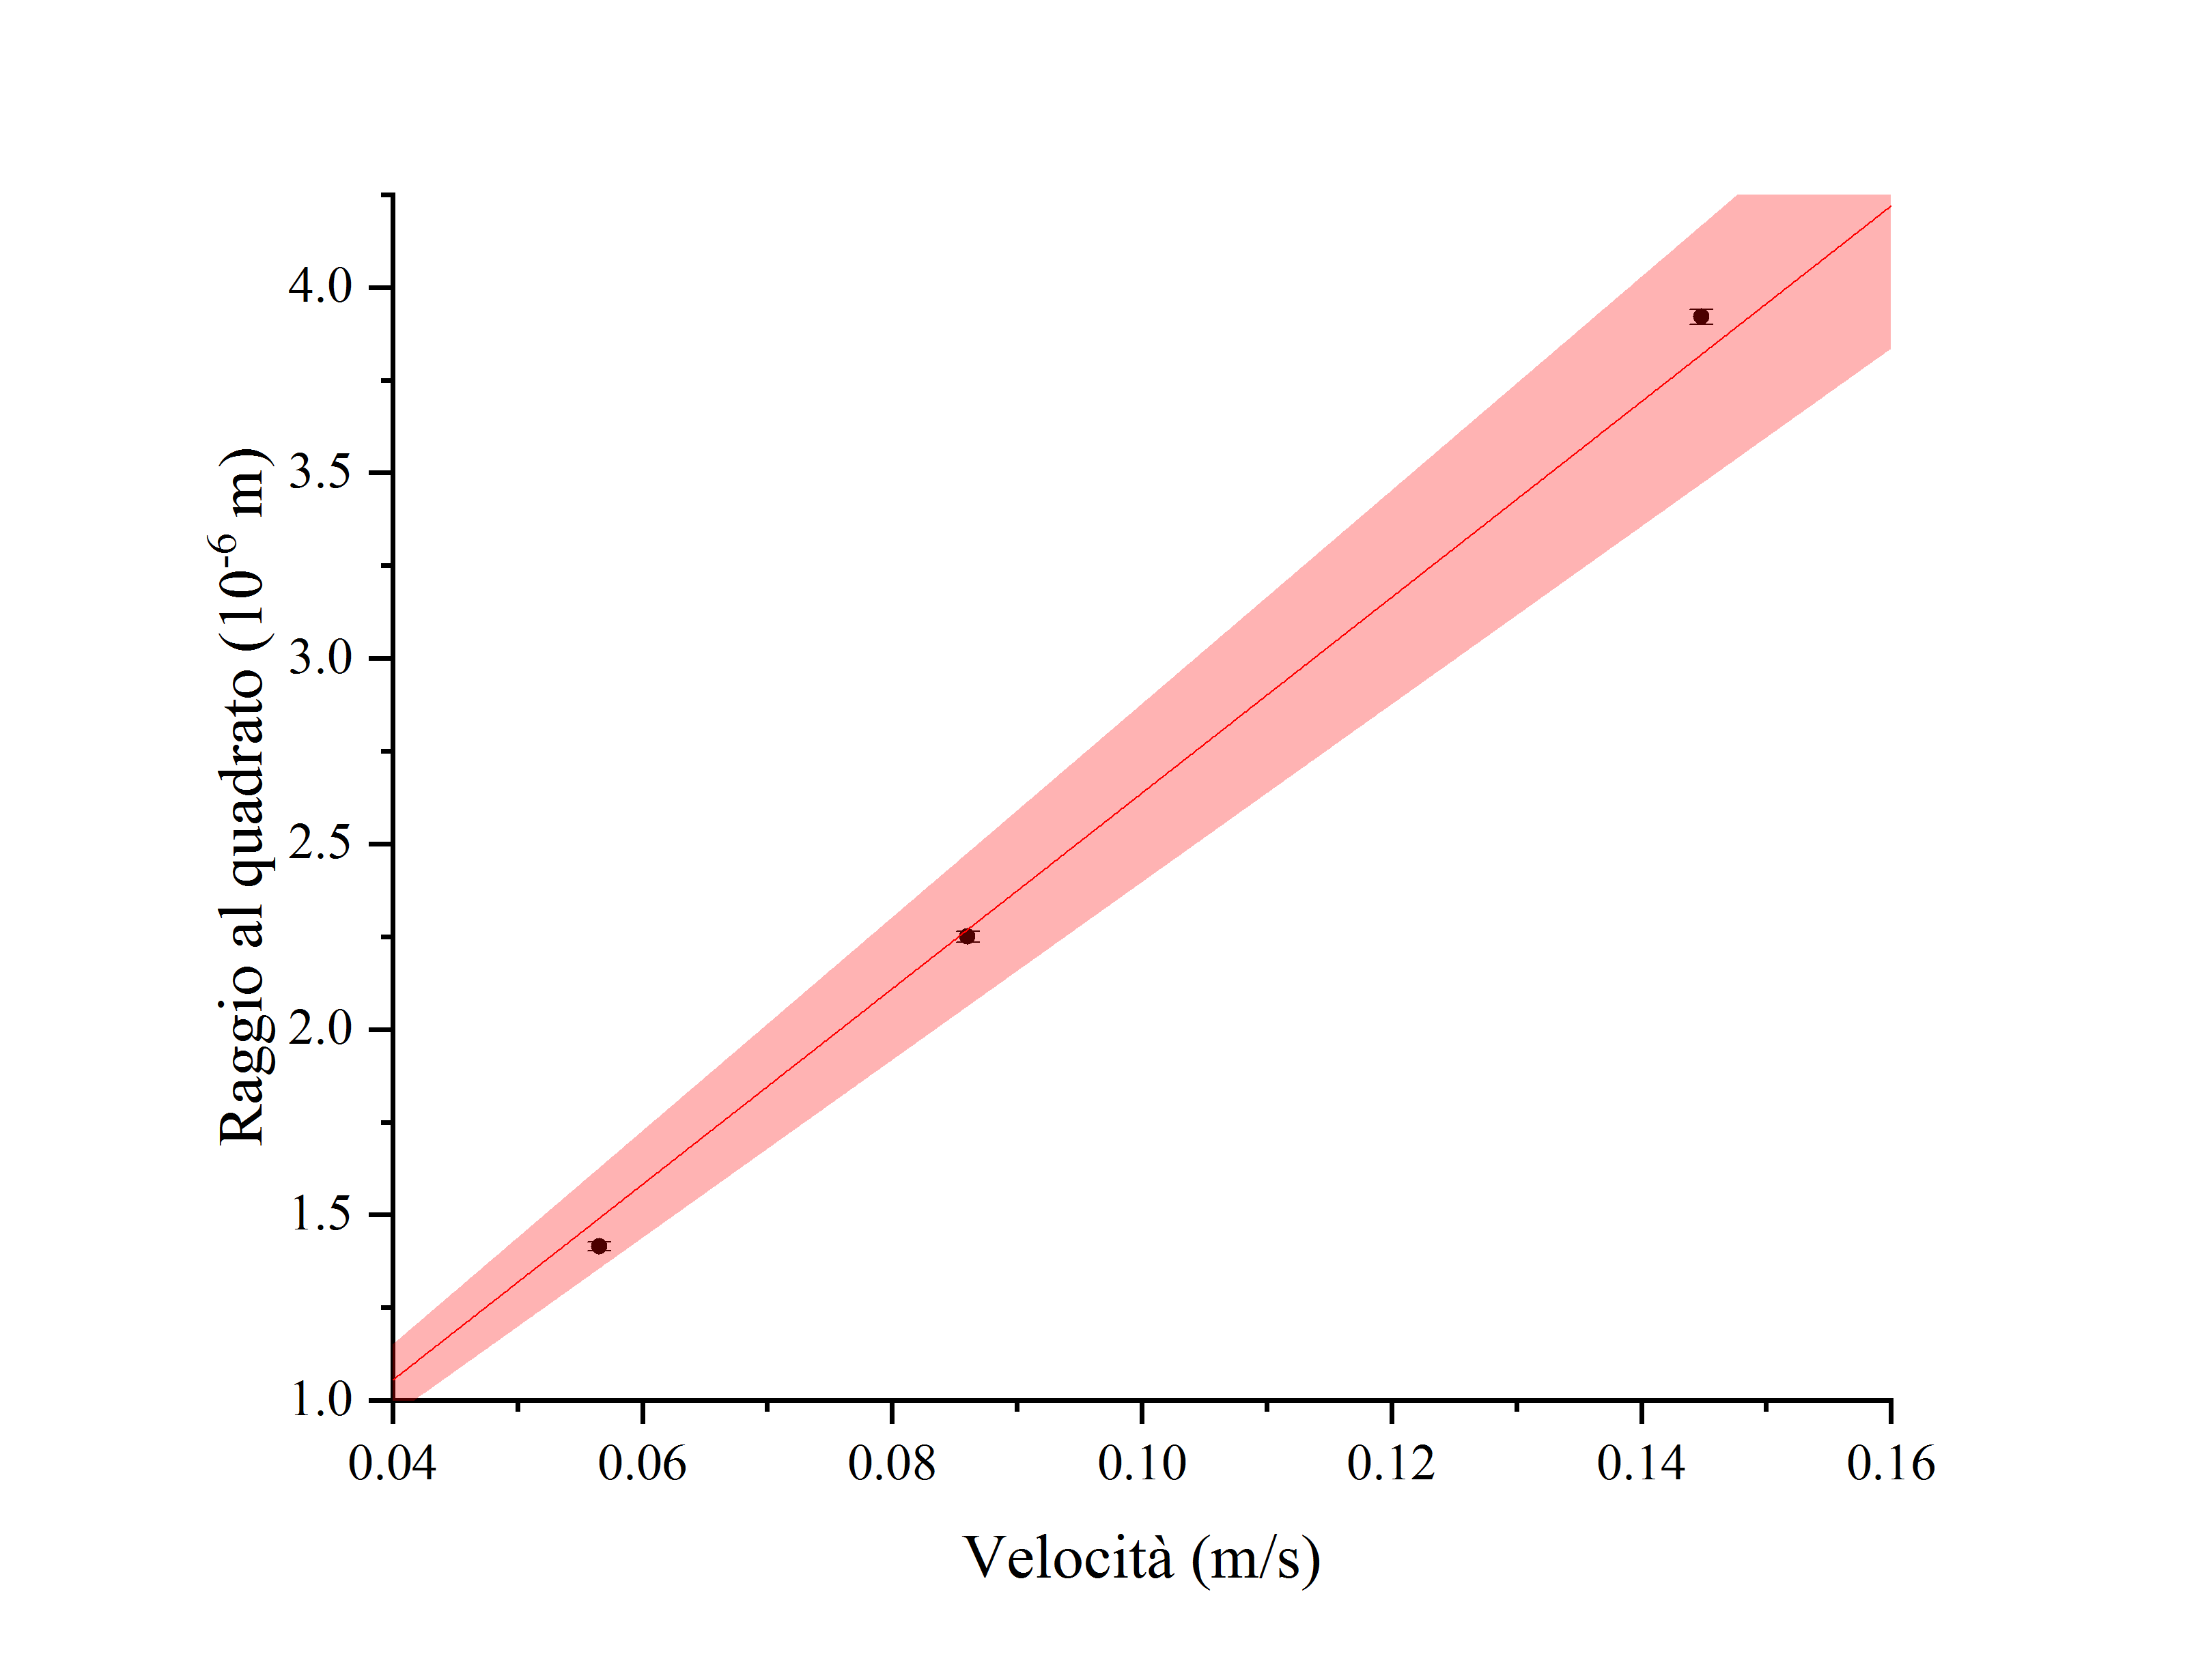
\includegraphics[trim={2.5cm 0.6cm 3cm 2.5cm},clip,width=.49\textwidth]{img/reg2.png}}
  \caption*{\emph{
    In rosso le rette di regressione, in rosa le rispettive
    regioni di incertezza.
    Le barre di errore in entrambe le direzioni sono riportate,
    ma sono troppo ridotte per poter essere apprezzate
    immediatamente.
  }}
\end{figure}

Per calcolare una prima stima di $\eta$ è possibile approssimare
$\rho_\text{sol}\simeq\rho_\text{glicerina}$, calcolata in base
a $T_\text{amb}$ secondo il modello sopra citato:
\[
  \eta = \frac{2g(\rho_\text{sf} - \rho_\text{sol})}{9\xi}
  \simeq \frac{2g(\rho_\text{sf} -
    \rho_\text{glicerina}(T_\text{amb}))}{9\xi}
\]
I valori di $\eta$ calcolati sulla base dei dati raccolti nelle
due giornate sono:
\[\eta_1=(256\pm3)\,\unit{mPa\,s}\qquad\qquad\eta_2=(371\pm4)\,\unit{mPa\,s}\]

\subsection{Concentrazione della glicerina}

Il modello empirico della viscosità di una soluzione acquosa di
glicerina è descritto dalla seguente equazione:
\[
  \eta_\text{sol} =
    \eta_\text{acqua}^\alpha \eta_\text{glicerina}^{1-\alpha}
\]
al variare di un parametro $\alpha\in[0,1]$ legato alla
concentrazione dell'acqua. Risolvendo l'equazione in $\alpha$ si
ottiene:
\[
  \alpha = \frac{\ln{\eta_\text{sol}} - \ln{\eta_\text{glicerina}}}
    {\ln{\eta_\text{acqua}} - \ln{\eta_\text{glicerina}}}
\]
La relazione tra $\alpha$ e la concentrazione in massa $c_\text{m}$
della \emph{glicerina} in soluzione è invece la seguente:
\[
  \alpha = 1 - c_\text{m} + \frac{a b\,c_\text{m} (1 - c_\text{m})}
    {a\,c_\text{m} + b (1 - c_\text{m})}
  \qquad\text{con}\quad
  \begin{array}{l}
    a = 0.705 - 0.0017\,T_\text{amb} \\
    b = (4.9 + 0.036\,T_\text{amb})\,a^{2.5}
  \end{array}
\]
Risolvendo l'equazione in $c_\text{m}$ si ottiene:
\[
  c_\text{m} = \frac{
    -\alpha a + \alpha b + ab + a - 2b - \sqrt{\Delta}}{2(ab + a - b)}
\]
con $
\Delta = \alpha^2 a^2 - 2\alpha^2 ab + \alpha^2 b^2 - 2\alpha a^2 b -
2\alpha a^2 - 2\alpha a b^2 + 2\alpha ab + a^2 b^2 + 2a^2 b + a^2$.

\vspace{2mm}
I valori di $\alpha$ e $c_\text{m}$ calcolati a partire da $\eta$ e
$T_\text{amb}$ per entrambi i giorni sono:
\[
\begin{aligned}
  \alpha_1 &= 0.174\pm0.006
  \qquad\qquad
  c_{\text{m},1} &= (93.6\pm0.3)\%\,\text{m}/\text{m}\\
  \alpha_2 &= 0.184\pm0.006
  \qquad\qquad
  c_{\text{m},2} &= (93.2\pm0.3)\%\,\text{m}/\text{m}\\
\end{aligned}
\]

\subsection{Ricalcolo della densità per una migliore stima}
Nota la concentrazione di glicerina, è ora possibile
calcolare una stima della densità della soluzione, facendo
ancora una volta affidamento ad un modello empirico:
\[
  \rho_\text{sol} = \kappa(T,c_\text{m}) \left(
  \rho_\text{acqua}(T) + \frac{
    \rho_\text{glicerina}(T) - \rho_\text{acqua}(T)
  }{1 + \frac{\rho_\text{glicerina}(T)}{\rho_\text{acqua}(T)}
    \!\left(\frac{1}{c_\text{m}} - 1\right)}
  \right)
\]
dove $
  \kappa(T,c_\text{m}) = 1 + \left(
    1.78\cdot10^{-6}\,T^2 - 1.82\cdot10^{-4}\,T + 1.41\cdot10^{-2}
  \right)\sin{\!\left(c_\text{m}^{1.31} \pi\right)}^{0.81}
$ è il coefficiente di espansione volumica.
% TODO: Spiegare chi è \kappa correttamente

Applicando questa formula ai valori di $T$ e $c_\text{m}$ di cui
sopra, otteniamo:
\[
  \rho_{\text{sol},1} = (1241.5\pm1.2)\,\unit{kg \per m^2}
  \qquad\qquad
  \rho_{\text{sol},2} = (1243.7\pm1.2)\,\unit{kg \per m^2}
\]

Possiamo osservare facilmente che queste misure non sono compatibili
con i rispettivi valori di $\rho_\text{glicerina}$: l'approssimazione
$\rho_\text{sol} \simeq \rho_\text{glicerina}$ non è quindi
giustificata.

Tuttavia, è evidente che:
\[(\rho_\text{sol})_\text{best} < (\rho_\text{glicerina})_\text{best}\]

Possiamo dunque immaginare che il $\rho_\text{sol}$ così determinato
approssimi il valore vero \emph{meglio} di $\rho_\text{glicerina}$.

Il gruppo di lavoro ha quindi deciso di ricalcolare la densità della
soluzione come appena mostrato, utilizzando stavolta la nuova stima di
$\rho_\text{sol}$.

\vspace{2mm}

Reiterando questo processo più volte, le stime di
$\rho_\text{sol}$, $c_\text{m}$ ed $\eta_\text{sol}$ si sono
velocemente stabilizzate attorno a valori ben definiti:
di seguito riportiamo i risultati delle prime iterazioni.

\begin{center}\begin{tblr}{
  colspec={ |c|c|c|c|c| }
}
  \hline
  \textbf{Giorno 1}
    & $\rho_\text{sol}\;(\unit{kg\per m^3})$
    & $\eta_\text{sol}\;(\unit{mPa\,s})$ & $c_\text{m}\;(\%\,\text{m}/\text{m})$
    & $\rho_\text{sol}\;(\unit{kg\per m^3})$
    \\ Iterazione & (assunto) &&& (ottenuto) \\
  \hline
  1 & $1257.94\pm0.12$ & $256.42\pm2.99$ & $93.56\pm0.26$ & $1241.53\pm1.21$ \\
  \hline[dashed]
  2 & $1241.53\pm1.21$ & $257.08\pm3.03$ & $93.58\pm0.26$ & $1241.57\pm1.21$ \\
  \hline[dashed]
  3 & $1241.57\pm1.21$ & $257.07\pm3.03$ & $93.58\pm0.26$ & $1241.57\pm1.21$ \\
  \hline[dashed]
  4 & $1241.57\pm1.21$ & $257.07\pm3.03$ & $93.58\pm0.26$ & $1241.57\pm1.21$ \\
  \hline[dashed]
  $\vdots$ & $\vdots$ & $\vdots$ & $\vdots$ & $\vdots$ \\
\end{tblr}\end{center}
\begin{center}\begin{tblr}{
  colspec={ |c|c|c|c|c| }
}
  \hline
  \textbf{Giorno 2}
    & $\rho_\text{sol}\;(\unit{kg\per m^3})$
    & $\eta_\text{sol}\;(\unit{mPa\,s})$ & $c_\text{m}\;(\%\,\text{m}/\text{m})$
    & $\rho_\text{sol}\;(\unit{kg\per m^3})$
    \\ Iterazione & (assunto) &&& (ottenuto) \\
  \hline
  1 & $1261.13\pm0.12$ & $370.80\pm4.32$ & $93.17\pm0.25$ & $1243.73\pm1.17$ \\
  \hline[dashed]
  2 & $1243.73\pm1.17$ & $371.80\pm4.38$ & $93.18\pm0.25$ & $1243.77\pm1.17$ \\
  \hline[dashed]
  3 & $1243.77\pm1.17$ & $371.80\pm4.38$ & $93.19\pm0.25$ & $1243.77\pm1.17$ \\
  \hline[dashed]
  4 & $1243.77\pm1.17$ & $371.80\pm4.38$ & $93.19\pm0.25$ & $1243.77\pm1.17$ \\
  \hline[dashed]
  $\vdots$ & $\vdots$ & $\vdots$ & $\vdots$ & $\vdots$ \\
\end{tblr}\end{center}
\begin{center}
  \emph{
    \textbf{Nota.}
    Abbiamo riportato più cifre decimali del necessario,
    semplicemente per mostrare le piccole differenze tra
    le prime iterazioni.
  }
\end{center}

\section{Conclusioni}



\pagebreak
I risultati della regressione lineare sono chiaramente compatibili
con i valori attesi. Infatti:
\begin{itemize}
  \item Secondo il modello fisico utilizzato, l'intercetta dovrebbe
  essere nulla; in effetti, $(0.003\pm0.005)\;\unit{m}$ è compatibile
  con $\qty{0}{m}$.
  \item Il valore di $g$ atteso è $\qty{9.806}{m\per s^2}$; si può
  osservare facilmente che il valore misurato,
  $(9.68\pm0.13)\;\unit{m \per s^2}$, è compatibile con esso.
\end{itemize}

Possiamo pertanto concludere che l'esperienza ha avuto successo:
mediante l'apparato sperimentale abbiamo ottenuto una misura di $g$
compatibile con quella attesa.

\pagebreak
Come è possibile osservare comparando questi risultati a
quelli precedentemente ottenuti, il valore di $g$ risultante
è rimasto essenzialmente invariato (al netto della sua incertezza).

In conclusione, possiamo affermare ragionevolmente che,
rispetto alla sensibilità degli strumenti di misura,
il contributo dell'attrito è trascurabile.

\end{document}
